
\chapter{Perimeter Guarding}
\thispagestyle{myheadings}

This chapter studies the problem of optimally assigning a larger number of sensing
robots (or other types of autonomous agents) to guard the perimeters of closed 2D regions,
where the perimeter of each region to be guarded may contain multiple disjoint polygonal chains.
The problem is termed ``perimeter guarding''.
We first introduce perimeter guarding with homogeneous sensors,
then step into perimeter guarding with heterogeneous sensors (~\ref{fig:intro-opg-he}). 

\section{Perimeter Guarding with Homogeneous Defenders}

\def\R{\mathcal R}
\def\C{\mathcal C}
\def\S{\mathcal S}
\def\P{\mathcal P}
\def\G{\mathcal G}
\def\W{\mathcal W}
%\thickmuskip=0mu
\def\opg{{\sc {OPG}}\xspace}

\subsection{Introduction}


\def\R{\mathcal R}
\def\C{\mathcal C}
\def\S{\mathcal S}
\def\P{\mathcal P}
\def\G{\mathcal G}
\def\W{\mathcal W}
%\thickmuskip=0mu
\def\opg{{\sc {OPG}}\xspace}

Consider the scenario from ~\ref{fig:opg-example}, which contains a closed region with its boundary (or border) demarcated by the red and dotted blue lines. To secure the region, either from intrusions from the outside or unwanted escapes from within, it is desirable to deploy a number of autonomous agents to monitor or guard either the entire boundary or selected portions of it (e.g., the red line segments), with each agent responsible for a continuous section. 
%
Naturally, one might also want to have even coverage by the agents, e.g., minimizing the maximum effort from any agent. In practice, such efforts may correspond to sensing ranges or motion capabilities of robots, which are always limited. 
%
As an intuitive example, the figure may represent the top view of a castle, with its entire boundary being a high wall that may be traversed by agents. 
%
The portion of the wall marked with the three red line segments must be protected, whereas the art marked by the dotted blue lines may not need active monitoring (e.g., the outside may be a cliff or a body of deep water). The green and orange lines show an optimal distribution of the workload by $8$ agents that cover all red segments but skip two of the three-dotted line segments. 

More formally, in this paper, we study the problem of deploying a large 
number of robots to guard a set of one-dimensional boundary segments 
called perimeters. Each perimeter is comprised of one or more 1D segments 
that are part of a circular boundary (e.g., the red segments in 
~\ref{fig:opg-example}). Each robot is tasked to guard a continuous 1D 
segment that covers a portion of a perimeter. As the main objective, 
we seek an allocation of robots such that {\em (i)} the union of the 
robots' coverage encloses all perimeters and {\em (ii)} the 
maximum coverage of any robot is minimized. We call this 1D deployment
problem the Optimal Perimeter Guarding (\opg) problem. 
\begin{figure}[ht]
\vspace*{0mm}
\begin{center}
\begin{overpic}[width=0.7\textwidth,tics=5]{./chapters/opg/figures/example.eps}
%\put(26,20){{\small $R_1$}}
%\put(20,39){{\small \textcolor{red}{$P_1$}}}
%\put(66,28){{\small $R_2$}}
%\put(54,40){{\small \textcolor{green}{$P_2$}}}
%\put(82,44){{\small $\W$}}
\end{overpic}
\end{center}
\vspace*{-5mm}
\caption{\label{fig:opg-example} An illustrative scenario where a perimeter, 
in this case represented as the red line segments, must be guarded by 
$n = 8$ robots, which are constrained to 
only travel along the perimeter boundary (the red line segments plus the 
dotted blue lines, which are gaps that do not need to be guarded). An 
optimal set of locations for the $8$ robots and the coverage region for 
each robot are marked on the perimeter boundary in green and orange, 
which minimizes the maximum coverage required for any robot.}
\vspace*{-8mm}
\end{figure}


In this work, three main \opg variants are examined. The settings 
regarding the perimeter in these three variants are: {\em (i)}
multiple perimeters with each having a single connected component; 
{\em (ii)} a single perimeter containing multiple connected components; 
and {\em (iii)} multiple perimeters with each containing multiple 
connected components (the most general case). For all three variants, 
we have developed exact algorithms for solving \opg that runs in low
polynomial time. More specifically, let there be $n$ robots, $m$ 
perimeters, with perimeter $i$ ($1 \le i \le m$) containing $q_i$ 
connected components. If $m = 1$, then let the only perimeter contains
$q$ connected components. For the three variants, our algorithm 
computes an optimal solution in time $O(m(\log n + \log m) + n)$, 
$O(q^2\log(n+q) + n)$, and $O((\sum_{1\le i \le m} q_i^2) \log(n + 
\sum_{1\le i \le m} q_i) + n)$, respectively, which
are roughly quadratic in the worst case. 
In addition to computing locations for deploying the robots, we 
further compute shortest paths for deploying the robots, given some 
initial configuration of the robots. The modeling of the \opg 
problem and the development of the efficient algorithms for \opg 
constitute the main contribution of this paper. 

With an emphasis on robotic swarm deployment, within multi-robot 
systems research \cite{arai2002advances,gerkey2004formal,ren2008distributed,bullo2009distributed}, 
our study is closely related to {\em formation control}, e.g., 
\cite{ando1999distributed,jadbabaie2003coordination,olfati2004consensus,ren2005consensus,cheng2008almost,mesbahi2010graph,yu2012rendezvous},
where the goal is to achieve certain {\em distributions} through 
continuous (often, local sensing based) interactions among the 
agents or robots. Depending on the particular setting, the 
distribution in question may be spatial, e.g., rendezvous
\cite{ando1999distributed,yu2012rendezvous}, or maybe an agreement 
in agent velocity is sought \cite{jadbabaie2003coordination,ren2005consensus}. 
In these studies, the resulting formation often have some 
degree-of-freedoms left unspecified. For example, rendezvous 
results \cite{ando1999distributed,yu2012rendezvous} often come 
with exponential convergence guarantee, but the location of
rendezvous is generally unknown {\em a priori}. 

On the other hand, in multi-robot task and motion planning problems (e.g.,
\cite{smith2009monotonic,ayanian2010decentralized,liu2011multi,liu2013optimal,turpin2014goal,turpin2014capt,alonso2015multi,SolYu15}), 
especially ones with a {\em task allocation} element 
\cite{smith2009monotonic,liu2011multi,liu2013optimal,turpin2014goal,turpin2014capt,SolYu15},
the (permutation-invariant) target configuration is often mostly 
known. The goal here is finding a one-to-one mapping between individual 
robots and the target locations (e.g., deciding a {\em matching}) and 
then plan (possibly collision-free) trajectories for the robots to reach 
their respective assigned targets \cite{turpin2014goal,turpin2014capt,SolYu15}.  
In contrast to formation control and multi-robot motion planning research, 
our study of \opg seeks to determine an exact, optimal distribution 
pattern of robots (in this case, over a fairly arbitrary, bounded 1D 
topological domain). Thus, solutions to \opg may serve as the target 
distributions for multi-robot task and motion planning, which is a main 
motivation behind our work. The generated distribution pattern is 
also potentially useful in multi-robot persistent monitoring 
\cite{soltero2014decentralized} and coverage \cite{howard2002mobile,schwager2009optimal} 
applications, where robots are asked to carry out sensing tasks in some 
optimal manner. 
	
As a multi-robot coverage problem, \opg is intimately connected to Art 
Gallery problems \cite{o1987art,shermer1992recent}, with origins traceable 
to half a century ago \cite{klee1969every}. Art Gallery problems assume 
a visibility-based \cite{lozano1979algorithm} sensing model; in a typical 
setup \cite{o1987art}, the {\em interior} of a polygon must be visible to at 
least one of the guards, which may be placed on the boundaries, corners, 
or the interior of the polygon. Finding the optimal number of guards are 
often NP-hard \cite{lee1986computational}. Alternatively, disc-based sensing 
model may be used, which leads to the classical {\em packing} problem 
\cite{thue1910dichteste,hales2005proof}, where no overlap is allowed between 
the sensors' coverage area, the {\em coverage} problem 
\cite{drezner1995facility,cortes2004coverage,pavone2009equitable,martinez2010distributed,pierson2017adapting}, 
where all 
workspace must be covered with overlaps allowed, or the {\em tiling} problem 
\cite{kershner1968paving}, where the goal is to have the union of sensing
ranges span the entire workspace without overlap. For a more complete 
account on Art Gallery, packing, and covering, see Chapters 2, 3, and 33 of
\cite{toth2017handbook}. Despite the existence of a large body of literature 
performing extensive studies on these intriguing computational geometry 
problems, these types of research mostly address domains that are 2D and 
higher. To our knowledge, \opg, as an optimal coverage problem over 
a non-trivial 1D topological space, represents a practical and novel formulation 
yet to be fully investigated. 

The rest of the chapter is organized as follows. 
%
The \opg problem and some of its most basic properties are described 
in Section~\ref{section:opg-problem}. 
%
In Section~\ref{section:opg-analysis}, a thorough structural analysis of \opg 
with single and multiple perimeters is performed, paving the way for 
introducing the full algorithmic solutions in Section~\ref{section:opg-algorithm}.
%
Then, in Section~\ref{section:opg-evaluation}, comprehensive numerical 
evaluations of the multiple polynomial-time algorithms are carried out. 
In addition, two realistic application scenarios are demonstrated. 
%
In Section~\ref{section:opg-conclusion}, we conclude with  
additional discussions. 


\subsection{The Optimal Perimeter Guarding Problem}\label{section:opg-problem}

Let $\W \subset \mathbb R^2$ be a compact (i.e., closed and bounded) 
two-dimensional workspace. There are  $m$ pairwise disjoint {\em 
regions} $\R = \{R_1, \ldots, R_m\}$ where each region $R_i \subset \W$ 
is homeomorphic to the closed unit disc, i.e., there exists a continuous 
bijection $f_i: R_i \to \{(x, y) \mid x^2 + y^2 \le 1\}$ for all $1 \le 
i \le m$. For a given region $R_i$, let $\partial R_i$ be its (closed) 
boundary (therefore, $f_i$ maps $\partial R_i$ to the unit circle  
$\mathbb S^1$). With a slight abuse of notation, define $\partial \R 
= \{\partial R_1, \ldots, \partial R_m\}$. Let $P_i \subset \partial R_i$ 
be the part of $\partial R_i$ that is accessible, e.g., not blocked by 
obstacles in $\W$. This means that each $P_i$ is either a single closed 
curve or formed by a finite number of (possibly curved) line segments. 
Define  $\P = \{P_1, \ldots, P_m\} \subset \W$ as the {\em perimeter} 
of $\R$ which must be {\em guarded}. More formally, each $P_i$ is 
homeomorphic to a compact subset of the unit circle (i.e., it is 
assumed that the maximal connected components of $P_i$ are closed 
line segments). For a given $P_i$, each one of its maximal connected 
component is called a {\em perimeter segment} or simply a {\em segment}, 
whereas each maximal connected components of $\partial R_i \backslash P_i$ 
is called a {\em perimeter gap} or simply a {\em gap}. An example setting is 
illustrated in ~\ref{fig:opg-example-boundaries} with two regions. 

\begin{figure}[ht]
\vspace*{-1mm}
\begin{center}
\begin{overpic}[width=0.7\textwidth,tics=5]
{./chapters/opg/figures/example-boundaries-eps-converted-to.pdf}
\put(26,20){{\small $R_1$}}
\put(20,39){{\small \textcolor{red}{$P_1$}}}
\put(66,28){{\small $R_2$}}
\put(54,40){{\small \textcolor{green}{$P_2$}}}
%\put(79.6,18){{\small $h$}}
\put(82,44){{\small $\W$}}
\end{overpic}
\end{center}
\vspace*{-4mm}
\caption[An example of a workspace $\W$ with two regions $\{R_1, R_2\}$]{\label{fig:opg-example-boundaries} An example of a workspace $\W$ 
with two regions $\{R_1, R_2\}$. Due to three {\em gaps} on $\partial R_1$, 
marked as dotted lines within long rectangles, $P_1 \subset \partial R_1$ 
has three {\em segments} (or maximal connected components); $P_2 = \partial 
R_2$ has a single segment with no gap.}
\vspace*{-3mm}
\end{figure}

There are $n$ indistinguishable point robots residing in $\W$.
%and outside of any $R_i \in \R$, $1 \le i \le m$. 
These robots are to be deployed to {\em cover} the perimeter $\P$ such 
that each robot $1 \le j \le n$ is assigned a continuous closed subset 
$C_j$ of some $\partial R_i, 1 \le i \le m$. All of $\P$ must be 
{\em covered} by $\C$, i.e., 
%
$\bigcup_{P_i \in \P} P_i  \subset \bigcup_{C_j \in \C} C_j$,
%
which implies that elements of $\C$ need not intersect on their
interiors. Hence, it is assumed that any two elements of $\C$ may share 
at most their endpoints. Such a $\C$ is called a cover of $\P$. 

Given a cover $\C$, for a $C_j \in \C$, $1 \le j \le n$, let $len(C_j)$ 
denote its length (more formally, measure). It is desirable to minimize 
the maximum $len(C_j)$, i.e., the goal is to find a cover $\C$ such that 
the value 
%
$\max_{C_j \in \C} len(C_j)$
%
is minimized. This corresponds to minimizing the maximum workload for 
each robot or agent. The formal definition of the Optimal Perimeter 
Guarding (\opg) problem is provided as follows. 

\begin{problem}[Optimal Perimeter Guarding (\opg)] Given the perimeter 
$\P = \{P_1, \ldots, P_m\}$ of a set of 2D regions $\R =\{R_1, \ldots, 
R_m\}$, find a set of $n$ continuous line segments $\C^* = \{C_1^*, 
\ldots, C_n^*\}$ such that $\C^*$ covers $\P$, i.e., 
\begin{align}\label{eq:opg-coverage}
\bigcup_{P_i \in \P} P_i  \subset \bigcup_{C_j^* \in \C^*} C_j^*,
\end{align}
with the maximum of $len(C_j^*), 1 \le j \le n$ minimized, i.e., among all 
covers $\C$ satisfying~\eqref{eq:opg-coverage}, 
\begin{align}\label{eq:opg-objective}
\C^* = \underset{\C}{\mathrm{argmin}} \max_{C_j \in \C} len(C_j).
\end{align}
\end{problem}

Here, we introduce the technical assumption that the ratio between 
the length of $\partial \R$ and the length of $\partial \P$ is polynomial
in the input parameters. That is, the length of $\partial \R$ is not much 
bigger than the length of $\partial \P$ . 
The assumption makes intuitive sense as any 
gap should not be much bigger than the perimeter in pratice. We note 
that the assumption is not strictly necessary but helps simplify the 
correctness proof of some algorithms. 

Henceforth, in general, $\C^*$ is used when an optimal cover is meant 
whereas $\C$ is used when a cover is meant. We further define the optimal 
single robot coverage length as 
\begin{align}\label{eq:opg-l-star}
\vspace*{-1mm}
\ell^* = \min_{\C} \max_{C_j \in \C} len(C_j).
\vspace*{-1mm}
\end{align}

~\ref{fig:opg-example} shows an example of an optimal cover by $8$ robots 
of a perimeter with three components. Note that one of the three gaps 
(the one on the top area as part of the hexagon) is fully covered 
by a robot, which leads to a smaller $\ell^*$ as compared to other 
feasible solutions. This interesting phenomenon, which is 
actually a main source of the difficulty in solving \opg, is explored 
more formally in Section~\ref{section:opg-analysis} 
(Proposition~\ref{p:opg-max-no-exclusion}).

Given the \opg formulation, additional details on $\partial \R$ must 
be specified to allow the precise characterization of the computational 
complexity (of any algorithm developed for \opg). For this purpose, it 
is assumed that each $\partial R_i \in \partial \R$, $1 \le i \le m$, 
is a simple (i.e., non-intersecting and without holes) polygon with an 
input complexity $O(M_i)$, i.e., $\partial R_i$ has about $M_i$ vertices 
or edges. If an \opg has a single region $R$, then let $\partial R$ have 
an input complexity of $M$. Note that the algorithms developed in this 
work apply to curved boundaries equally well, provided that the curves 
have similar input complexity and are given in a format that allow the 
computation of their lengths with the same complexity. 
Alternatively, curved boundaries may be approximated to arbitrary 
precision with polygons. 

%\jy{Add an example showing an optimal cover for maybe some $6-10$ robots?
%This can probably go in the introduction to motivate the paper. We need 
%some 1-2 good examples. Need to refer back to the example here.}

For deploying a robot to guard a $C_j$, one natural choice is to send the 
robot to a location $t_j \in C_j$ such that $t_j$ is the centroid of $C_j$. 
Since $C_j$ is one dimensional, $t_j$ is the center (or midpoint) of $C_j$. 
After solving an \opg, there is the remaining problem of assigning the $n$ 
robots to the centers of $\C^* = \{C_j^*\}$ and actually moving the robots 
to these assigned locations. As a secondary objective, it may also be 
desirable to provide guarantees on the execution time required for 
deploying the robots to reach target guarding locations. We note that, 
the task assignment (after determining target locations) and motion 
planning component for handling robot deployment, essential for applications 
but not a key part of this work's contribution, is briefly addressed in 
Section~\ref{section:opg-evaluation}. 

With some $\C^*$ satisfying~\eqref{eq:opg-coverage} 
and~\eqref{eq:opg-objective}, we may further require that $len(C_j^*)$ is 
minimized for all $C_j^* \in \C^*$. This means that a gap $G \subset 
((\bigcup \partial R_i)\backslash (\bigcup P_i))$ will never be partially 
covered by some $C_j^* \in \C^*$ because if that is the case, $C_j^*$ 
needs not cover any part of $G$ at all (and should not, to limit the 
coverage of the assigned robot). In the example from 
~\ref{fig:opg-example-boundaries}, $G$ may be one of the three dotted 
lines on $\partial R_1$; clearly, it is not beneficial to have some 
$C_j^*$ partially cover (i.e., intersect the interior of) one of these. 
This rather useful condition (note that this is not an assumption but 
a solution property) yields the following lemma. 

\begin{lemma}\label{l:opg-no-partial-coverage} 
For a set of perimeters $\P = \{P_1,\ldots, P_m\}$ where $P_i \subset 
\partial R_i$ for $1 \le i \le m$, there exists an optimal cover $\C^* 
= \{C_1^*, \ldots, C_n^*\}$ such that, for any gap (or maximal connected
component) $G \subset ((\bigcup \partial R_i)\backslash (\bigcup P_i))$ 
and any $C_j^* \in \C^*$, $C_j^* \cap G = G$ or $C_j^* \cap G = 
\varnothing$. 
\end{lemma}

\begin{remark} Our definition of coverage is but one of the possible 
models of coverage. The definition restricts a robot deployed to 
$C_j, 1 \le j \le n$, to essential {\em live} on $C_j$. The definition 
models scenarios where a guarding robot must travel along $C_j$, which 
is one-dimensional. Nevertheless, the algorithms developed for \opg have 
broader applications. For example, subroutines in our algorithms readily 
solve the problem of finding the minimum number of guards needed if each 
guard has a predetermined maximum coverage. 
%As we will demonstrate later, by selecting the 
%boundaries (i.e., $\{\partial R_i\}$) carefully, the model applies 
%to diverse practical application scenarios.
\end{remark}


\subsection{Structural Analysis}\label{section:opg-analysis}
In designing efficient algorithms, the solution structure of \opg induced by 
the problem formulation is first explored, starting from the case where there 
is a single region.

\subsubsection{Guarding a Single Region}
\noindent\textbf{Perimeter with a single connected component}. For 
guarding a single region $\R = \{R\}$, i.e., there is a single 
boundary $\partial R$ to be guarded, all $n$ robots can be directly 
allocated to $\partial R$. If the single perimeter $P \subset 
\partial R$ further has a single connected component that is either 
homeomorphic to $\mathbb S^1$ or $[0, 1]$, then each robot $j$ can 
be assigned a piece $C_j \subset P$ such that $\bigcup_{C_j \in \C} 
C_j = P$ and $len(C_j) = len(P)/n$. Clearly, such a cover $\C$ is 
also an optimal cover. 

\noindent\textbf{Perimeter with multiple maximal connected components}. 
When there are multiple maximal connected components (or segments) in a 
single perimeter $P$, things become more complex. To facilitate the 
discussion, assume here $P$ has $q$ segments $S_1, \ldots, S_q$ arranged 
in the clockwise direction (i.e., $P = S_1 \bigcup \ldots \bigcup S_q$), 
which leaves $q$ gaps $G_1, \ldots, G_q$ with $G_k$ immediately following 
$S_k$. Fig.~\ref{fig:single-perimeter} shows a perimeter with five segments
and five gaps. 
\begin{figure}[ht]
\vspace*{-1mm}
\begin{center}
\begin{overpic}[width=0.7\textwidth,tics=5]
{./chapters/opg/figures/single-perimeter.eps}
\put(16,7){{\small $S_1$}}
\put(17,31){{\small $G_1$}}
\put(46,30){{\small $S_2$}}
\put(56.5,28){{\small $G_2$}}
\put(72,27.5){{\small $S_3$}}
\put(84.5,17.5){{\small $G_3$}}
\put(85,6){{\small $S_4$}}
\put(72,-4){{\small $G_4$}}
\put(59,0){{\small $S_5$}}
\put(45,4){{\small $G_5$}}
\end{overpic}
\end{center}
\vspace*{-1mm}
\caption{\label{fig:single-perimeter} A perimeter $P$ with five segments 
$S_1, \ldots, S_5$, separated by five {\em gaps} $G_1, \ldots, G_5$.}
\vspace*{-3mm}
\end{figure}

Suppose an optimal set of assignments for the $n$ robots guarding $P$ 
and  satisfying~\eqref{eq:coverage} and~\eqref{eq:objective} is $\C^* 
= \{C_j^*\}$. Let $G_{max}$ be a largest gap, i.e., $len(G_{max}) = 
\max_{1 \le k \le q}len(G_k)$. Via small perturbations to the lengths 
of $G_k$, we may also assume that $G_{max}$ is unique. If we exclude 
the gap $G_{max}$ and have the $n$ robots cover the rest of $\partial 
R$ evenly, then it must hold that $len(C_j^*) \le (len(\partial R) - 
len(G_{max}))/n$. On the other hand, $len(C_j^*) \ge (\sum_{1\le k\le 
q}len(S_k))/n$ always holds. These yield a pair of basic upper and 
lower bounds for the optimal single robot coverage length $\ell^*$, 
summarized as follows. 

\begin{proposition}\label{p:single-bounds} Define 
\[
\ell_{min} = \frac{\sum_{1\le k\le q}len(S_k)}{n}\,\,and\,\,
\ell_{max} = \frac{len(\partial R) -  len(G_{max})}{n},
\]
it holds that 
\begin{align}\label{eq:lopt} 
\ell_{min} \le \ell^* \le \ell_{max}.
\end{align}
\end{proposition}

On the other hand, it is not always the case that a largest gap $G_{max}$, 
even if unique, will be skipped by $\bigcup_{C_j \in \C^*} C_j^*$. 
That is, an optimal cover $C^*$ may enclose the largest gap. 
 
\begin{proposition}\label{p:max-no-exclusion}
Given a region $R$ and perimeter $P \subset \partial R$, let
$G_{max}$ be the unique longest connected component of $\partial R
\backslash P$. Let $\C^*$ be an optimal cover of $P$. Then, it is 
possible that $G_{max} \subset C_j^*$ for some $C_j^* \in \C^*$. 
\end{proposition}
\begin{proof}The claim may be proved via contradiction with the example 
illustrated  in Fig.~\ref{fig:max-not-skipped} which readily generalizes. 
In the figure, there are four gaps $G_1, \ldots, G_4$, in which three 
gaps ($G_1$, $G_2$, and $G_4$) have the same length (i.e., $len(G_1)= 
len(G_2)= len(G_4)$) and are evenly spaced (i.e., $len(S_1)= len(S_2) 
= len(S_3\cup G_3\cup S_4)$). Here, $G_{max} = G_3$, which is 
$1.5$ times the length of other gaps, i.e., $len(G_3) = 
\frac{3}{2}len(G_1)$. 
\begin{figure}[ht]
\vspace*{0mm}
\begin{center}
\begin{overpic}[width=0.7\textwidth,tics=5]{./chapters/opg/figures/max-not-skipped.eps}
\put(27,34){{\small $S_1$}}
\put(48,44){{\small $G_1$}}
\put(69,34){{\small $S_2$}}
\put(69,9){{\small $G_2$}}
\put(62,1){{\small $S_3$}}
\put(48,-4){{\small $G_3$}}
\put(32,2){{\small $S_4$}}
\put(26,8){{\small $G_4$}}
\end{overpic}
\end{center}
\vspace*{-3mm}
\caption{\label{fig:max-not-skipped} A case where the perimeter has 
four segments or maximal connected components. Three of the gaps, 
$G_1$, $G_2$, and $G_4$ are of the same length and are evenly spaced, 
$G_3$ is $0.5$ times longer.}
\vspace*{-3mm}
\end{figure}

For $n = 3$ robots, the optimal cover $\C^*$ must allocate each robot 
to guard each of $S_1$, $S_2$, and $(S_3\cup G_3\cup S_4)$. Without 
loss of generality, let $C_1^* = S_1$, $C_2^* = S_2$, and $C_3^* = 
(S_3\cup G_3\cup S_4)$. This means that $G_3$ is covered by $C_3^*$ 
and not skipped by $\C^*$. In this case, $len(C_1^*) =len(C_2^*) = 
len(C_3^*) = len (S_1)$.

To see that this must be the case, suppose on the contrary that $G_3$ 
is skipped and let $\C = \{C_1, C_2, C_3\}$ be an alternative cover. 
By Lemma~\ref{l:no-partial-coverage}, an optimal cover must skip $G_3$ 
entirely. In this case, some $C_j$, say $C_1$, must have its left end 
point\footnote{In this paper, for a non-circular segment or gap, its 
left end point is defined as the {\em limit point} along the 
counterclockwise direction along the perimeter and its right end point 
is defined as the limit point in the clockwise direction along the 
perimeter. So, in Fig.~\ref{fig:max-not-skipped}, for $S_1$, its left 
end point touches $G_4$ and its right end point touches $G_1$.} coincide 
with the right end point of of $G_3$ (the point where $G_3$ meets $S_4$). 
Then $C_1$ must cover $S_4$ and $G_4$; otherwise, $C_2$ and $C_3$ must 
cover $S_1 \cup S_2 \cup S_3$, which makes $len(C_2) + len(C_3) \ge 
len(S_1 \cup S_2 \cup S_3) > 2len(S_1)$ and $\C$ a worse cover than 
$\C^*$. By symmetry, similarly, some $C_j$, say $C_3$, must have its 
right end point coincide with the left end point of $G_3$ and cover 
$S_3$ and $G_2$. However, this means that both $G_2$ and $G_4$ are 
covered by $\C$. Even if $G_1$ is skipped, this makes $len(C_1 \cup 
C_2 \cup C_3) = len(S_4 \cup G_4 \cup S_1 \cup S_2 \cup G_2 \cup S_3) 
> len (S_1 \cup S_2 \cup S_3\cup G_3\cup S_4) > 3len(S_1)$, again making
$\C$ sub-optimal. By the pigeonhole principle, at least one of the $C_1$, 
$C_2$, or $C_3$ must be longer than $len(S_1)$. Therefore, skipping 
$G_{max} = G_3$ in this case leads to a sub-optimal cover. The only 
other alternative for an optimal cover with $n = 3$ is to have $C^* = 
\{S_1, S_2, (S_3\cup G_3\cup S_4)\}$. 
\end{proof}

Proposition~\ref{p:max-no-exclusion} implies that in allocating robots 
to guard a perimeter $P \subset \partial R$, an algorithm cannot simply 
start by excluding the longest component from $\partial R 
\backslash P$ and then the next largest, and so on. This makes solving
\opg more challenging. Referring back to Fig.~\ref{fig:example}, if the 
top gap is skipped by the cover, then the three robots on the right side 
of the perimeter (two orange and one green) need to cover the part of the 
perimeter between the two hexagons. This will cause $\ell^*$ to increase. 

On the other hand, for an optimal cover $\C^* = \{C_1^*, \ldots, C_n^*\}$ 
of $P$, some $C_j^*\in \C^*$ must have at least one of its end point 
aligned with an endpoint of a component $S_k$ of $P$ (assuming that $P 
\subsetneq \partial R$). 

\begin{proposition}\label{p:endpoint-alignment}
For an optimal cover $\C^* = \{C_1^*,\ldots, C_n^*\}$ of a perimeter 
$P = S_1 \bigcup \ldots \bigcup S_q \subset \partial R = S_1 \bigcup G_1 
\bigcup $ $\ldots \bigcup S_q \bigcup G_q$, for some $S_i \subset P$ and 
$C_j^* \in C^*$, their right (or left) endpoints must coincide. 
\end{proposition}
\begin{proof}
By Lemma~\ref{l:no-partial-coverage}, for any $G_k \subset \partial R 
\backslash P$, and $C_j^* \in \C^*$, $G_k \cap C_j^* = G_k$ or 
$G_k \cap C_j^* = \emptyset$. Since at least one $G_k$, $1 \le k \le q$, 
must be skipped by $C_1^* \cup \ldots C_n^*$, some $C_j^*$, $1 \le j \le n$ 
must have its right endpoint aligned with the right endpoint of $S_k$, 
which is on the left of $G_k$. Following the same argument, some 
$C_{j'}^*$ and $S_{k'}$ must have the same left endpoints. 
\end{proof}

Proposition~\ref{p:endpoint-alignment} suggests that we may attempt to cover 
a perimeter $P$ starting from an endpoint of $S_1$, $S_2$, and so on. 
%An algorithm can attempt a binary search approach to first test whether 
%$\ell^* \le \frac{\ell_{min} + \ell_{max}}{2}$ or $\ell^* > \frac{\ell_{min} 
%+ \ell_{max}}{2}$. For each candidate of $\ell^*$, we need to try at most $q$ 
%left starting points for $C_1$. This yields an algorithm that allows the 
%approximation of $\ell^*$ arbitrarily well for a given $P$ and $n$.  
Indeed, as we will show in Section~\ref{section:algorithm}, an efficient 
algorithm can be designed exploiting this important fact. 


\subsubsection{Guarding Multiple Regions}
In a multiple region setup, there is one additional level of complexity:
the number of robots that will be assigned to an individual region is 
no longer fixed. This introduces another set of variables $n_1, \ldots, 
n_m$ with $n_1 + \ldots + n_m = n$ and $n_i$, $1 \le i \le m$ being the 
number of robots allocated to guard $\partial R_i$. For a fixed $n_i$, 
the results derived for a single region, i.e., 
Propositions~\ref{p:single-bounds}--\ref{p:endpoint-alignment} continue 
to hold.



\subsection{Efficient Algorithms for Perimeter Guarding}\label{section:opg-algorithm}
\def\algoMRSimple{{\sc MultiRegionSingleComp}\xspace}
\def\algoSRG{{\sc SingleRegionMultiComp}\xspace}
\def\algoMRG{{\sc MultiRegionMultiComp}\xspace}
\def\isLFeasible{{\sc IsFeasible}}
\def\isLFeasibleByTilingPartial{{\sc IsTilingFeasiblePartial}}
\def\isLFeasibleByTilingFull{{\sc IsTilingFeasibleFull}}
%
In presenting algorithms for \opg, we begin with the case 
where each perimeter $P_i \in \P$ has a single connected component 
(i.e., $P_i$ is homeomorphic to $\mathbb S^1$ or $[0, 1]$). Then, 
we work on the general single region case where the only perimeter 
is composed of $q > 1$ connected components, before moving to the 
most general multiple regions case.

\subsection{Perimeters Containing Single Components}
When there is a single perimeter $P$, the solution is straightforward 
with $\ell^* = len(P)/n$. With $\ell^*$ determined, $\C^*$ is also readily computed. 

In the case where there are $m > 1$ regions, let the optimal 
distribution of the $n$ robots among the $m$ regions are given by 
$n_1^*, \ldots, n_m^*$. For a given region $R_i$, the $n_i^*$ robots 
must each guard a length $\ell_i = len(P_i)/n_i^*$. At this point, we
observe that for at least one region, say $R_i$, 
the corresponding $\ell_i$ must be maximal, i.e., $\ell_i = \ell^*$. 
The observation directly leads to a naive strategy for finding $\ell^*$: 
for each $R_i$, one may simply try all possible $1 \le n_i \le n$ and 
find the maximum $len(P_i)/n_i$ that is feasible, i.e., $n - n_i$ robots
can cover all other $R_{i'}$, $i' \ne i$, with each robot covering no 
more than $len(P_i)/n_i$. Denoting this $len(P_i)/n_i$ as $\ell_i^c$ and 
the corresponding $n_i$ as $n_i^c$, the smallest $\ell_i^c$ overall $1 
\le i \le m$ is then $\ell^*$.

The basic strategy mentioned above works and runs in polynomial time. 
However, it is possible to carry out the computation much more 
efficiently if the longest $P_i$ is examined first. Without loss of 
generality, assume that $P_1$ is the longest perimeter, i.e., $len(P_1)
\ge len(P_{i})$ for all $1 \le i \le m$. Recall that $n_1^c$ is the 
number of robots allocated to $P_1$ that yields $\ell_1^c$, it must hold 
that 
\begin{align}\label{eq:opg-l1}
\frac{len(P_1)}{n_1^c + 1} < \ell^* \le \frac{len(P_1)}{n_1^c} = \ell_1^c .
\end{align}
For an arbitrary $P_i$, simple manipulating of~\eqref{eq:opg-l1} yields
\begin{align}\label{eq:opg-li}
\frac{len(P_i)}{(n_1^c + 1)\frac{len(P_i)}{len(P_1)}} < \ell^* \le 
\frac{len(P_i)}{n_1^c\frac{len(P_i)}{len(P_1)}}.
\end{align}
This means that we only need to consider
$
n_i^c \in 
\big[\lceil n_1^c\frac{len(P_i)}{len(P_1)} \rceil, 
\lfloor (n_1^c + 1)\frac{len(P_i)}{len(P_1)}\rfloor].
$
However, since $P_1$ is the longest perimeter, $\frac{len(P_i)}{len(P_1)} 
\le 1$. Therefore, the difference between the two denominators 
of~\eqref{eq:opg-li} is no more than $1$, i.e., 
\[
(n_1^c + 1)\frac{len(P_i)}{len(P_1)} - n_1^c\frac{len(P_i)}{len(P_1)} \le 1. 
\]
When $len(P_i) \ne len(P_1)$, $(n_1^c + 1)\frac{len(P_i)}{len(P_1)} 
- n_1^c\frac{len(P_i)}{len(P_1)} < 1$ and there are two possibilities. One 
of these is 
$
\lceil n_1^c\frac{len(P_i)}{len(P_1)} \rceil =
\lfloor (n_1^c + 1)\frac{len(P_i)}{len(P_1)}\rfloor,
$
which leaves a single possible candidate for $n_i^c$. The other 
possibility 
is 
$
\lceil n_1^c\frac{len(P_i)}{len(P_1)} \rceil =
\lfloor (n_1^c + 1)\frac{len(P_i)}{len(P_1)}\rfloor + 1,
$
in which case there is actually no valid candidate for $n_i^c$. 
That is, after computing $n_1^c$ and $\ell_1^c$, if $len(P_i) = len(P_i)$ 
then no computation is needed for $P_i$. If $len(P_i) < len(P_1)$ then we 
only need to check at most one candidate for $n_i^c$. 

%The observation directly leads to an algorithm for computing $\ell^*$: 
%for each $P_i$, $1 \le i \le m$, we test all possible $1 \le n_i \le n 
%- m + 1$ (the rest of the $m -1$ regions need at least $m -1$ guards) 
%and for a fixed $n_i$ compute a candidate $\ell_i =  len(P_i)/n_i$. 
%This $\ell_i$ is assumed to be a potential $\ell^*$, which should be 
%the largest single robot coverage. Then, we check whether $n - n_i$ 
%robots can cover all perimeters except $P_i$ where each robot cannot 
%have coverage larger than $\ell_i$. For all feasible $1 \le n_i \le n$,
%the one that yields the smallest $\ell_i$ is kept. Denote this pair of 
%$n_i$ and $\ell_i$ as $n_i^{c}$ and $\ell_i^{c}$ where the superscript 
%means ``candidate''. Then, the smallest $\ell_i^{c}$ over all 
%$1 \le i \le m$ must be the desired $\ell^*$. 

Additional heuristics can be applied to reduce the required computation. 
First, in finding $n_1^c$, we may use bisection (binary search) over 
$[1, m]$ since if a given $n_1$ is infeasible, any $n_1' < n_1$ cannot 
be feasible either because $len(P_1)/n_1 < len(P_1)/n_1'$. Second, let 
$\ell = (\sum_{1\le i\le m}len(P_i))/n$, it holds that $\ell_i^c \ge 
\ell^* \ge \ell$. This means that for each $1 \le i \le m$, it is not 
necessary to try any $n_i > \lfloor \frac{len(P_i)}{\ell} \rfloor$. 
Third, if a candidate $\ell_i^c$ is at any time larger than the current 
candidate for $\ell^*$, that $i$ does not need to be checked further. 
We only use the first and the third in our implementation since the 
second does not help much once the bisection is applied. The 
pseudo code is outlined in Algorithm~\ref{algo:opg-MRS}. Note that we 
assume the problem instance is feasible ($n \ge m$), which is easy to check. 

It is straightforward to verify that Algorithm~\ref{algo:opg-MRS} runs in 
time $O(m\log n + m^2)$. The $O(m\log n)$ comes from the $\mathbf{while}$ 
loop, which calls the function \isLFeasible($\ell_i^c$, $n_i^c$, $i$) 
$\log n$ time. The function checks whether the current $\ell_i^c$ is 
feasible for perimeters other than $P_i$ (note that it is assumed that 
\isLFeasible($\cdot$) has access to the input to Algorithm~\ref{algo:opg-MRS} 
as well). This is done by computing for $i' \ne i$, $n_{i'} = \lceil 
len(P_{i'})/\ell_i^c \rceil$ and checking whether $\sum_{{i'} \ne i}n_{i'} 
\le n - n_i^c$. The $O(m^2)$ term comes from the $\mathbf{for}$ loop. 
The running time of Algorithm~\ref{algo:opg-MRS} may be further reduced by 
noting that the $\mathbf{for}$ loop examines $(m-1)$ candidate 
$\ell_i^c$. These $\ell_i^c$ can be first computed and sorted, on which 
bisection can be applied. This drops the main running time to 
$O(m(\log n + \log m))$. This second bisection is not reflected in 
Algorithm~\ref{algo:opg-MRS} to keep the logic and notation more 
straightforward. If we also consider input complexity, an additional 
$O(\sum_{1\le i \le m} M_i)$ is needed to compute $len(P_i)$ from the raw polygonal 
input and an additional $O(n)$ time is needed for generating the actual
locations for the $n$ robots. The total complexity is then $O(m(\log n + 
\log m) + \sum_{1\le i \le m} M_i + n)$.
%\sh{Algorithm style: 
%(1) Change displaystyle to remove small font.
%(2) Tighten up by using lIf instead of If.}
%\jy{We can do some of these if needed. I used this style for some 
%particular reason that I can tell you :).}
% \vspace*{-3mm}

\begin{algorithm}[H]
	\SetKwInOut{Input}{Input}
	\SetKwInOut{Output}{Output}
	\SetKwComment{Comment}{\%}{}
	\setstretch{0.8}
\begin{small}
	\Input{$P_1, \ldots, P_m$: each $P_i$ a continuous polygonal line; 
		assume that $P_1$ is a longest perimeter \\
		$n$: the number of robots}
	\Output{$\ell^*, i^*$: the optimal coverage and the $i$ realizing it}
	\vspace{0.025in}

	$\ell^* \leftarrow \infty$; $i^* \leftarrow 1$;
	\vspace{0.025in}

	\Comment{\footnotesize Compute $n_1^c$ and initial $\ell^*$.}

	$n_1^{min} \leftarrow 1$; $n_1^{max} \leftarrow n$; $n_1^c \leftarrow 1$;
	\vspace{0.025in}

	\While{$n_1^{min} \ne n_1^{max}$}{
	\vspace{0.025in}
	$n_1 \leftarrow \lceil \frac{n_1^{min} + n_1^{max}}{2} \rceil$;
	$\ell_1 \leftarrow \frac{len(P_1)}{n_1}$;

	\vspace{0.025in}
	\uIf{\isLFeasible($\ell_1$, $n_1$, $1$)}{
		\vspace{0.025in}
		$\ell^* \leftarrow \ell_1$; 
		$n_1^c \leftarrow n_1$;
		$n_1^{min} \leftarrow n_1$; 
	}
	\Else{
		$n_1^{max} \leftarrow n_1 - 1$; 
	}
	}

	\vspace{0.05in}
	\Comment{\footnotesize Optimize $\ell^*$ over all $2 \le i \le m$.}


	\For{$i \in \{2,\dots, m\}$ }{\label{algo:opg-mrs:for}
		$n_i^- = \lceil \frac{n_1^clen(P_i)}{len(P_1)} \rceil$;
		$n_i^+ = \lfloor \frac{(n_1^c +1)len(P_i)}{len(P_1)} \rfloor$; 
		$\ell_i \leftarrow \frac{len(P_i)}{n_i^+}$;
					
			\If{$n_i^- == n_i^+$ and \isLFeasible($\ell_i$, $n_i^+$, $i$) and $\ell_i < \ell^*$}{
				\vspace{0.025in}
				$\ell^* \leftarrow \ell_i$; $i^* \leftarrow i$;
			}
	}
	\Return{$\ell^*$, $i^*$}
\end{small}
	\caption{\algoMRSimple} \label{algo:opg-MRS}
\end{algorithm}
% \vspace*{-6mm}


\subsection{Single Perimeter Containing Multiple Components}
In computing $\ell^*$ for a single perimeter $P$ with multiple connected 
components, assume that $P$ is composed of $q$ maximal connected 
components $S_1, \ldots, S_q$ (e.g., ~\ref{fig:opg-single-perimeter}),
leaving $G_1, \ldots, G_q$ as the gaps on $\partial R$. Given an 
optimal cover $\C^* = \{C_1^*, \ldots, C_n^*\}$, by 
Proposition~\ref{p:opg-endpoint-alignment}, we may assume that the left
end point of some $C_j^*$, $1 \le j \le n$ coincides with the left 
end point of some $S_k$, $1 \le k \le q$. We then look at the right 
end point of $C_j^*$. If it does not coincide with the right end point 
of some $S_{k'}$ ($k$ and $k'$ may or may not be the same), it must 
coincide with the left end point of $C_{j+1}^*$. Continuing like this, 
eventually we will hit some $C_{j'}^*$ where the right end point of 
$C_{j'}^*$ coincides with the right end point of some $S_{k'}$. 
Within a partitioned subset $C_j^*, \ldots, C_{j'}^*$, the coverage of 
each robot is minimized when $len(C_j^*) = \ldots = len(C_{j'}^*)$. 
Because $\ell^* = len(C_j^*)$ for some $1 \le j \le n$, at least one 
of the subsets must have all robots cover exactly a length of $\ell^*$. 
These two key observations are summarized as follows. 

\vspace*{-1mm}
\begin{theorem}\label{t:opg-optimal-partition}
Let $\C^* = \{C_1^*, \ldots, C_n^*\}$ be a solution to an \opg instance
with a single perimeter $P = S_1\cup \ldots\cup S_q$ and gaps $G_1, \ldots, 
G_q$. Then, $\C^*$ may be partitioned into disjoint subsets with
the following properties
\begin{enumerate}
\item the union of the individual elements from any subset forms a 
continuous line segment, 
\item the left end point of such a union coincides with the left end 
point of some $S_k$, $1 \le k \le q$, 
\item the right end point of such a union coincides with the right end 
point of some $S_{k'}$, $1 \le k' \le q$,  and
\item the respective unions of elements from any two subsets are 
disjoint, i.e., they are separated by at least one gap. 
\end{enumerate}
Moreover, for at least one such subset, $\{C_j^*, \ldots, C_{j'}^*\}$, 
it holds that $\ell^* = len(C_j^*) = \ldots = len(C_{j'}^*)$. 
\vspace*{-1mm}
\end{theorem}

\noindent\textbf{A baseline algorithm}.
In the example from ~\ref{fig:opg-example}, $\C^*$ is partitioned into 
two subsets satisfying the conditions stated in 
Theorem~\ref{t:opg-optimal-partition}. The theorem provides a way for 
computing $\ell^*$. For fixed $1 \le k, k' \le q$, denote the part of 
$\partial R$ between $S_k$ and $S_{k'}$ following a clockwise direction 
(with $S_k$ and $S_{k'}$ included) as $S_{k-k'}$.
Theorem~\ref{t:opg-optimal-partition} says that for some $k, k'$, $len(S_{k-k'})
= n_{k-k'}^*\ell^*$ for some integer $n_{k-k'}^* \in [1, n]$. We may 
find $k', k'$, and $n_{k-k'}^*$, $\ell^*$ by exhaustively going through all 
possible $k, k'$, and $n_{k-k'}^c$ (as a candidate of $n_{k-k'}^*$). For 
each combination of $k, k'$ and $n_{k-k'}^c$, we can compute a 
\begin{align}\label{eq:opg-lkkc}
\vspace*{-2mm}
\ell_{k-k'}^c = \frac{len(S_{k-k'})}{n_{k-k'}^c}
\vspace*{-2mm}
\end{align}
and check $\ell_{k-k'}^c$'s feasibility. The largest feasible 
$\ell_{k-k'}^c$ is $\ell^*$. 

For checking feasibility of a particular $\ell_{k-k'}^c$, i.e., whether 
$\ell_{k-k'}^c$ is long enough for the rest of the robots to cover the 
rest of the perimeter, we simply {\em tile} $(n - n_{k-k'}^c)$ copies 
$\ell_{k-k'}^c$ over the rest of the perimeter, starting from $S_{(k' 
\mod q) + 1}$. As an example, see ~\ref{fig:opg-tiling} where $n = 6$ 
robots are to cover the perimeter (in red, with five components $S_1, 
\ldots, S_5$). Suppose that the algorithm is currently working with 
$S_{1-2}$ (i.e., $k=1$ and $k' = 2$). If  $n_{1-2}^c = 2$, then 
$\ell_{1-2}^c = len(S_{1-2})/2$. Each of the five green line segments 
$C_1, \ldots, C_5$  in the figure has this length. As visualized in the 
figure, it is possible to cover $P\backslash S_{1-2}$ with three more 
robots, which is no more than $n - n_{1-2}^c = 4$. Therefore, this 
$\ell_{1-2}^c$ is feasible; note that it is not necessary to exhaust 
all $n = 6$ robots. In the figure, $C_3$ covers the entire $S_3$ and 
$G_3$, as well as part of $S_4$. The rest of $S_4$ is covered by $C_4$. 
As $C_4$ is tiled, it ends in the middle of $G_4$, so $C_5$ starts at 
the beginning of $S_5$. 
%
On the other hand, if $n_{1-2}^c = 3$, the resulting $\ell_{1-2}^c$ 
(each of the orange line segments has this length) is infeasible as part 
of $S_5$ is now left uncovered.
\begin{figure}[ht]
	\vspace*{-2mm}
	\begin{center}
		\begin{overpic}[width=0.6\textwidth,tics=5]{./chapters/opg/figures/tiling.eps}
			\put(13,2.7){{\small $S_1$}}
			\put(27,2.7){{\small $S_2$}}
			\put(45,2.7){{\small $S_3$}}
			\put(60,2.7){{\small $S_4$}}
			\put(86.5,2.7){{\small $S_5$}}
			\put(12.5,10){{\small $C_1$}}
			\put(25,10){{\small $C_2$}}
			\put(48,10){{\small $C_3$}}
			\put(61,10){{\small $C_4$}}
			\put(86.5,10){{\small $C_5$}}
			%\put(54,40){{\small \textcolor{green}{$P_2$}}}
			%\put(82,44){{\small $\W$}}
		\end{overpic}
	\end{center}
	\vspace*{-4.5mm}
	\caption{\label{fig:opg-tiling}  An illustration of the feasibility check of 
		$\ell_{1-2}^c$. The single rectangular region and the perimeter (five red 
		segments $S_1$--$S_5$) are shown at the bottom. The orange and green line 
		segments show two potential	covers.}
	\vspace*{-3mm}
\end{figure}

The tiling-based feasibility check takes $O(q)$ time since there are at 
most $q$ segments to tile; it takes constant time to tile each segment 
using a given length. Let us denote this feasibility check 
\isLFeasibleByTilingPartial($k$, $k'$, $n_{k-k'}^c$), we have obtained 
an algorithm that runs in $O(nq^3)$ times since it needs to go through 
all $1 \le k \le q$, $1 \le k' \le q$, and $1 \le n_{k-k'}^c \le n$ and 
for each combination of $k, k'$, and $n_{k-k'}^c$, it makes a call to 
\isLFeasibleByTilingPartial($\cdot$). While a $O(nq^3)$ running time 
is not bad, we can do significantly better. 

\noindent\textbf{A much faster algorithm}.
In the baseline algorithm, for each $k-k'$ combination, up to $n$ 
candidate $n_{k-k'}^c$ may be attempted. To gain speedups, the first 
phase of the improved algorithm reduces the range of $\ell^*$ to limit 
the choice of $n_{k-k'}^c$. As a necessity, a feasibility check given 
only a length $\ell$ is introduced. That is, given an $\ell$, a check
is done to see whether $n$ robots are sufficient for covering $P$. 
This feasibility check is performed in a way similar to the tiling process from 
\isLFeasibleByTilingPartial($\cdot$) but now $k$ and $k'$ are not 
specified. Therefore, we need to try all $S_k$, $1 \le k \le q$ as the 
possible starting segment for the tiling. Let us denote this procedure
\isLFeasibleByTilingFull($\ell$), which runs in $O(q^2)$.

With \isLFeasibleByTilingFull($\ell$), starting from the initial bounds 
for $\ell^*$ given in Proposition~\ref{p:opg-single-bounds}, we can narrow the
bound to be arbitrarily small, using bisection, since $\ell^*$ is the 
minimum feasible $\ell$. To do this, we start with $\ell$ as the middle 
point of initial lower bound $\ell_{min}$ and upper bound $\ell_{max}$, 
and run \isLFeasibleByTilingFull($\ell$). If $\ell$ is feasible, the upper bound 
is lowered to $\ell$. Otherwise, the lower bound is raised to $\ell$. In doing 
this,  our goal in the first phase of the faster
algorithm is to reduce the range for $\ell^*$ so that there is only a 
constant number of choices for $n_{k-k'}^c$. We now derive when the 
bisection process should end. 
\setlength{\abovedisplayskip}{1.6pt}
\setlength{\belowdisplayskip}{2.0pt}
%\setlength{\abovedisplayskip}{4.2pt}
%\setlength{\belowdisplayskip}{4.2pt}

Assume that when the bisection ends, the lower and upper bounds are 
$\ell_{min}^f$ and $\ell_{max}^f$. Then, for some $\ell_{k-k'}^c$
(see~\eqref{eq:opg-lkkc}), it holds that
\[
\ell_{min}^f \le \ell_{k-k'}^c = \frac{len(S_{k-k'})}{n_{k-k'}^c} \le \ell_{max}^f.
\]
Rearranging the above yields
\[
\frac{len(S_{k-k'})}{\ell_{max}^f} \le n_{k-k'}^c \le \frac{len(S_{k-k'})}{\ell_{min}^f}.
\]
To reduce the number of possible $n_{k-k'}^c$ to at most $1$, we want 
\[
\frac{len(S_{k-k'})}{\ell_{min}^f} - \frac{len(S_{k-k'})}{\ell_{max}^f} < 1, 
\]
which is the same as requiring 
\begin{align}\label{eq:opg-lmmd}
\ell_{max}^f- \ell_{min}^f <
\frac{\ell_{max}^f\ell_{min}^f}{len(S_{k-k'})}. 
\end{align}
Noting that $\ell_{min}^f, \ell_{max}^f \ge  \ell_{min}$ and $len(S_{k-k'}) < 
len (\partial R)$, Equation~\eqref{eq:opg-lmmd} is ensured by 
\begin{align}\label{eq:opg-lmmd2}
\ell_{max}^f- \ell_{min}^f 
< \frac{\ell_{min}^2}{len(\partial R)} 
= \frac{\Big[\sum_{1\le k\le q}len(S_k)\Big]^2}{n^2len(\partial R)} 
\end{align}

Equation~\eqref{eq:opg-lmmd2} gives the stopping criteria used for refining 
the bounds for $\ell^*$. After completing the first phase, the faster algorithm
moves to the second phase of actually pinning down $\ell^*$. In this phase, 
instead of checking $\ell_{k-k'}^c$ one by one, we collect $\ell_{k-k'}^c$ for
all possible combinations of $k, k'$. Because the first phase already ensures
for each $k, k'$ combination there is at most one pair of $n_{k-k'}^c$ and 
$\ell_{k-k'}^c$, there are 
at most $q^2$ total candidates. After all candidates are collected, they are 
sorted and another bisection is performed over these sorted candidates. 
Feasibility check is done using \isLFeasibleByTilingPartial($\cdot$). The 
complete algorithm is given in Algorithm~\ref{algo:opg-SRG}. Note that 
$\ell^{min}$ and $\ell^{max}$, which change as the algorithm runs, are not 
the same as the fixed $\ell_{min}$ and $\ell_{max}$ from 
Proposition~\ref{p:opg-single-bounds}. 
\newpage
\vspace*{-7mm}
\begin{algorithm}
	\begin{small}
		\SetKwInOut{Input}{Input}
		\SetKwInOut{Output}{Output}
		\SetKwComment{Comment}{\%}{}
		\Input{$\partial R = S_1 \cup G_1 \cup \ldots \cup S_q \cup G_q$: a 
			single boundary with the perimeter $P = S_1 \cup \ldots \cup S_q$.\\
			$n$: the number of robots}
		\Output{$\ell^*, k^*, k'^{*}$: the optimal coverage and the 
			pair of $k$ and $k'$ that realize the optimal coverage}
		\vspace{0.025in}
		
		\Comment{\footnotesize Phase one: narrow the range of $\ell^*$.}
		$\ell^{min} \leftarrow \frac{\sum_{1\le k\le q}len(S_k)}{n}$, 
		$\ell^{max} \leftarrow  \frac{len(\partial R) -  len(G_{max})}{n}$;
		\vspace{0.025in}
		
		\While{$\ell^{max}-\ell^{min} > \frac{[\sum_{1\le k\le q}len(S_k)]^2}{n^2len(\partial R)}$}{
			$\ell \leftarrow \frac{\ell^{max}+\ell^{min}}{2}$;

			\vspace{0.025in}
			(\,\isLFeasibleByTilingFull($\ell$)? $\ell^{max} \leftarrow \ell$ : 
			$\ell^{min} \leftarrow \ell$\,);

			%\uIf{\isLFeasibleByTilingFull($\ell$)}{$\ell^{max} \leftarrow \ell$;}
			%\Else{$\ell^{min} \leftarrow \ell$;}
		}
		
		\vspace{0.025in}
		\Comment{\footnotesize Phase two: pin down $\ell^*$.}
		$sm \leftarrow []$; \Comment{$sm$ is a sorted map.}
		

		\For{$k, k' \in \{1,\dots, q\}$ }{\label{algo:opg-srg:for}
			\vspace{0.025in}
			
			$n_{k-k'}^{max} \leftarrow \lfloor \frac{len(S_{k-k'})}{\ell^{min}} \rfloor$;
			$n_{k-k'}^{min} \leftarrow \lceil \frac{len(S_{k-k'})}{\ell^{max}} \rceil$;
			
			\vspace{0.025in}
			
			\For{$n_{k-k'}^c \in \{n_{k-k'}^{min}, \ldots, n_{k-k'}^{max}\}$}{\label{algo:opg-srg:for2}
				$sm$.put($\frac{len(S_{k-k'})}{n_{k-k'}^c}$, $(n_{k-k'}^c, \frac{len(S_{k-k'})}{n_{k-k'}^c}, k, k')$);
			}
		}
	
		\vspace{0.025in}
		$\ell^* \leftarrow \infty$; $k^* \leftarrow 0$; $k'^* \leftarrow 0$;
		
		\vspace{0.025in}
		\While{$sm.\mathrm{size()}$ $> 1$}{
			\Comment{\footnotesize Extract the element from sm in the middle.}
			$(n^c, \ell^c, k, k') \leftarrow sm$.middleValue(); 
	
			\vspace{0.025in}
			\uIf{\isLFeasibleByTilingPartial($k, k', n^c$)}{
				$\ell^* \leftarrow \ell^c$; $k^* \leftarrow k$; $k'^* \leftarrow k'$;
				
				$sm \leftarrow sm.$range($sm.$minKey(), $\ell^c$);
			}
			\Else{
				$sm \leftarrow sm.$removeRange($sm.$minKey(), $\ell^c$);
			}
		}		
		
		\Return{$\ell^*$, $k^*$, $k'^*$}
		\caption{\algoSRG} \label{algo:opg-SRG}
	\end{small}
\end{algorithm}
\vspace*{-3mm}

In terms of running time, the first $\mathbf{while}$ loop starts with 
$\ell^{max} - \ell^{min} = \frac{len(\partial R) -  len(G_{max})}{n} -
\frac{\sum_{1\le k\le q}len(S_k)}{n} \le \frac{len(\partial R)}{n}$ and 
stops when $\ell^{max} - \ell^{min} \le 
\frac{[\sum_{1\le k\le q}len(S_k)]^2}{n^2len(\partial R)}$. Therefore, 
the bisection is executed 
$\log \frac{n[len(\partial R)]^2}{[\sum_{1\le k\le q}len(S_k)]^2}$ times, 
which by the assumption that $len(\partial R)$ is a polynomial factor over 
$\sum_{1\le k\le q}len(S_k)$, is $O(\log (n + q))$. Since each feasibility 
check takes $O(q^2)$ time, the first $\mathbf{while}$ loop takes 
$O(q^2\log(n + q))$ time. The $\mathbf{for}$ loops work with a total of 
$O(q^2)$ candidates and must sort them, taking time $O(q^2 \log q^2) = 
O(q^2 \log q)$. Then, the second $\mathbf{while}$ loop bisects $O(q^2)$ 
candidates and calls \isLFeasibleByTilingPartial($\cdot$) for each check, 
taking time $O(q\log q^2) = O(q\log q)$. The total running time of 
Algorithm~\ref{algo:opg-SRG} is then $O(q^2\log (n + q) + M + n)$.\footnote{We note that 
the assumption that $len(\partial R)$ is a polynomial factor over 
$\sum_{1\le k\le q}len(S_k)$ is not necessary. However, the corresponding 
analysis becomes much more involved without it. Since the assumption makes 
practical sense and also due to space limit, the more general result is 
omitted from the current paper. Many additional interesting but 
non-essential details, including this one, will be included in an extended 
version.}


\vspace*{-2mm}
\subsection{Multiple Perimeters Containing Multiple Components}
\vspace*{-1mm}
The algorithm for the multiple perimeter case is a direct 
generalization Algorithm~\ref{algo:opg-SRG}. To facilitate the description, 
let the perimeter $P_i$, $1 \le i \le m$, contain $q_i$ maximal connected 
components, i.e., $P_i = S_{i,1} \cup\ldots \cup S_{i,q_i}$ and the 
boundary $\partial R_i = S_{i,1} \cup G_{i,1} \cup \ldots \cup S_{i,q_i} 
\cup G_{i,q_i}$. We extend the definition of $S_{k-k'}$ for a single 
perimeter to $S_{i,k-k'}$ for multiple perimeters. By a straightforward 
generalization of Theorem~\ref{t:opg-optimal-partition} to multiple perimeters,
for an \opg instance, the length of some $S_{i,k-k'}$ must be an integer 
multiple of $\ell^*$. Similar to the single perimeter case, we can try 
all $S_{i,k-k'}$ and for each try all possible $1 \le n_{i,k-k'}^c \le n$. 
This gives us $\ell_{i,k-k'}^c = \frac{len(S_{i,k-k'})}{n_{i,k-k'}^c}$ as 
candidates for $\ell^*$; there are $n(\sum_{1\le i \le m} q_i^2)$ such 
candidates. For checking the feasibility of $\ell_{i,k-k'}^c$, we may use 
\isLFeasibleByTilingPartial($\cdot$) for the rest of $P_i$ (taking $O(q_i)$ 
time) and \isLFeasibleByTilingFull($\cdot$) for all $1 \le i' \le m$ and $i' 
\ne i$ (taking $O(\sum_{1 \le i' \le m, i' \ne i} q_{i'}^2)$ time). 
This yields a baseline algorithm that runs in 
$O(n(\sum_{1\le i \le m} q_i^2)^2)$ time. 

From here, speedups can be obtained as in the single perimeter case using 
the same reasoning. This yields a two-phase algorithm, which we call 
\algoMRG, that runs in $O((\sum_{1\le i \le m} q_i^2) \log(n + 
\sum_{1\le i \le m} q_i) + \sum_{1\le i \le m} M_i + n)$. 

%%
%The general strategy for computing $\ell^*$ remains the same: in this 
%case with multiple perimeters, some robots must still cover the optimal 
%length $\ell^*$ on some perimeter $P_i$. Following the basic reasoning, 
%each $P_i$ is checked to compute a $\ell_i^c$ that is a candidate for 
%$\ell^*$. Comparing all $\ell_i^c$ then yields $\ell^*$. For a fixed 
%$P_i$, computing $\ell_i^c$ is completed using a modified version of 
%Algorithm~\ref{algo:SRG} with the function \isLFeasibleByTilingPartial($\cdot$) 
%updated so it can handle multiple regions. 
%
%Assuming that a $P_i$ is fixed and $\ell_i^c$ is being computed. Before 
%\isLFeasibleByTilingPartial($\cdot$) is called, a candidate for $\ell_i^c$ (and 
%in turn a candidate for $\ell^*$), denoted $\ell_{i, k-k'}^c$ to include 
%an index for the perimeter, is computed. When called, 
%\isLFeasibleByTilingPartial($\cdot$) first does what it does in 
%Algorithm~\ref{algo:SRG}, which verifies that $\ell_{i, k-k'}^c$ works 
%for the rest of $P_i$ (e.g., the procedure explained with the example 
%around ~\ref{fig:tiling}). At this point, a total of $n_i^c$ robots 
%have been used to cover $P_i$, leaving $n - n_i^c$ robots to cover
%all perimeters other than $P_i$ such that no robot may cover more than
%$\ell_{i, k-k'}^c$. This can be achieved by finding the least number of 
%robots needed to cover each $P_{i'}$, $i' \ne i$ and check 
%the total is no more than $n - n_i^c$.
%
%To find the least number of robots needed to cover $P_{i'}$ such that 
%no robot covers more than $\ell_{i, k-k'}^c$, the same tiling strategy 
%is used. Unlike in the case for $P_i$, where the tiling starts from 
%the right end of $G_{i,k'}$, a left starting point for tiling is not 
%specified for $P_{i'}$. The straightforward thing to do is to try all 
%possible choices; there are $q_{i'}$ such possibilities. With this, the  
%algorithm for the general multiple perimeters case is fully specified. 
%Given the similarity of the algorithm to Algorithm~\ref{algo:SRG},
%an algorithm outline is omitted. For reference, we denote the algorithm 
%\algoMRG.
%
%To analyze the running time, we start with the updated
%\isLFeasibleByTilingPartial($\cdot$). Tiling of $P_i$ requires $O(q_i + n_i)$ 
%running time where $n_i$ is the number of robots that are needed to 
%cover $P_i$. Then, for any $P_{i'}$, $i'\ne i$, $q_{i'}$ locations on 
%$P_{i'}$ must be checked, each taking $O(q_{i'} + n_{i'})$ time, where 
%$n_{i'}$ is the number of robots needed to cover $P_{i}'$. The total time 
%spent by \isLFeasibleByTilingPartial($\cdot$) every time is then bounded by
%$O(q_i + n_i + \sum_{i' \ne i} (q_{i'}(q_{i'} + n_{i'})))$ which is 
%bounded by $O(\sum_{1 \le i \le m} q_{i}(n_{i} + q_{i}))$. Then, 
%checking all possible $k-k'$ combinations for $P_i$ (where $1 \le k, 
%k' \le q_i$) adds a multiplicative factor of $O(q_i (q_i + n_i))$. 
%Therefore, checking everything requires calling the routine
%\isLFeasibleByTilingPartial($\cdot$) about $O(\sum_{1 \le i \le m} 
%q_{i}(n_{i} + q_{i}))$ times. Similar to Algorithms~\ref{algo:MRS} 
%and~\ref{algo:SRG}, bisection may be applied here which makes the 
%total running time 
%\[
%O\big(\sum_{1 \le i \le m} \big[q_{i}(n_{i} + q_{i})\big]
%\log\big[\sum_{1 \le i \le m} q_{i}(n_{i} + q_{i})\big]\big),
%\]
%which is nearly quadratic. Again, if we consider input complexity, an
%additional $O(\sum_{1 \le i \le m} M_i)$ complexity needs to be added
%to the total. 
%



\subsection{Performance Evaluation and Applications}\label{section:opg-evaluation}
Our evaluation first verifies the algorithms' running time matches 
the claimed bounds. Then, two practical scenarios are illustrated 
to show how \opg may be adapted to applications. 

\vspace*{-1mm}
\subsection{Algorithm Performance}
\vspace*{-1mm}
In the performance results presented here, a data point is the 
average from $10$ randomly generated \opg instances. All algorithms 
are implemented in Python 2.7, and all experiments are executed on 
an Intel\textsuperscript{\textregistered} Xeon\textsuperscript{\textregistered} 
%E5-1660 v3 
CPU at 3.0GHz. % with 32GB RAM.% at 2133MHz.
Some additional performance results can be found in the Appendix.

%\subsubsection{\algoMRSimple} 
For the case of $m$ perimeters each containing a single segment, for 
each $1 \le i \le m$, we set $len(\partial R_i) = 1$ and let $len(P_i)$ 
be uniformly distributed in $(0, 1]$. ~\ref{fig:opg-mpsc-example} shows 
the result for an example with $m = 10$ and $n = 30$. For various values 
of $m, n$, the running time of \algoMRSimple is summarized in 
Table~\ref{eval:opg-mpsc}, which scales very well with $m$ and $n$ (note that 
the $n \le m$ case does not make much sense here). 

\begin{figure}[ht!]
    \vspace*{-3mm}
    \centering
    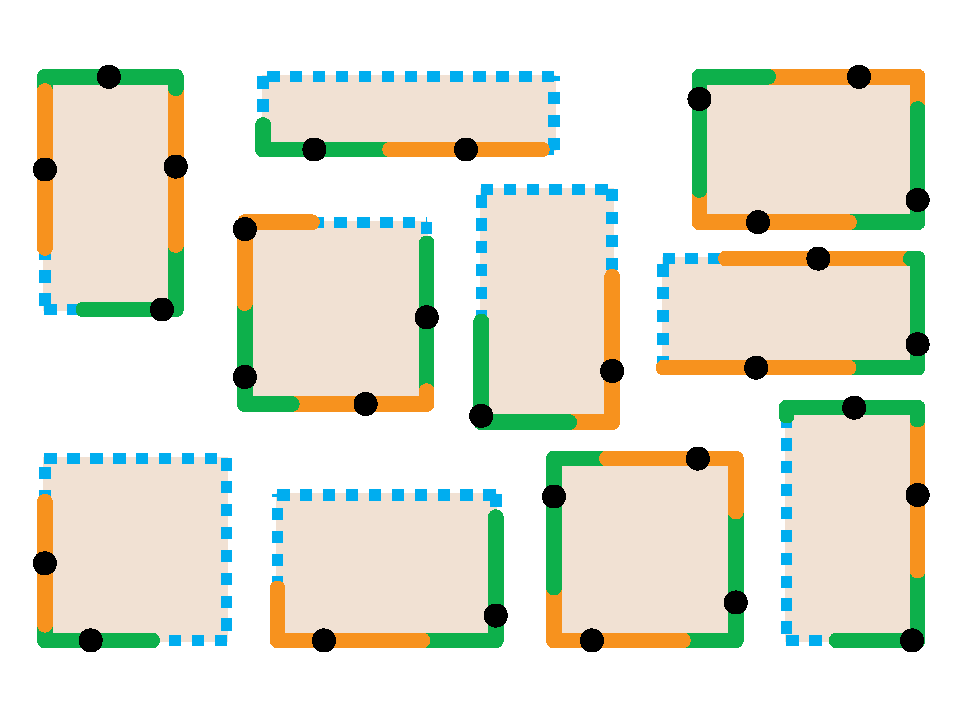
\includegraphics[keepaspectratio, scale=0.32]{./chapters/opg/figures/mpsc-example-eps-converted-to.pdf}
    \vspace*{-6mm}
    \caption[An example problem instance for MPSC]{\label{fig:opg-mpsc-example} 
    An example problem instance when $m = 10$ and $n = 30$. The black dots
		indicate deployed robot locations; the green and orange lines indicate
		the coverage.
    %We use blue dashed lines to show the gaps which do not need to be covered. 
    %The black filled circles illustrate final robot deployment locations, and 
    %the orange/green lines demonstrate individual robot covers. 
    %In this example, we use a different distribution to sample $len(P_i)$ due to 
    %cosmetic reasons.
		}
    \vspace*{-2mm}
\end{figure}

\begin{table}[ht!]
    \centering
		\vspace*{-4mm}
    \begin{footnotesize}
    \begin{tabular}{|c|c|c|c|c|c|c|} 
        \hline
        \diagbox{$m$}{$n$}       & $10^8  $ & $10^9   $ & $10^{10}$ & $10^{11}$ & $10^{12}  $ \\ \hline
        %\rule{0pt}{2.5ex} $10^3$ & $0.001 $ & $0.001  $ & $0.001  $ & $0.001  $ & $0.001    $ \\ \hline
        %\rule{0pt}{2.5ex} $10^4$ & $0.006 $ & $0.007  $ & $0.008  $ & $0.008  $ & $0.008    $ \\ \hline
        %\rule{0pt}{2.5ex} $10^5$ & $0.075 $ & $0.088  $ & $0.102  $ & $0.107  $ & $0.106    $ \\ \hline
        \rule{0pt}{2.5ex} $10^6$ & $1.152 $ & $1.442  $ & $1.508  $ & $1.652  $ & $1.617    $ \\ \hline
        \rule{0pt}{2.5ex} $10^7$ & $13.963$ & $17.281 $ & $18.796 $ & $20.354 $ & $20.627   $ \\ \hline
        \rule{0pt}{2.5ex} $10^8$ & NA       & $176.115$ & $223.186$ & $227.250$ & $230.000  $ \\ \hline
    \end{tabular}
		\end{footnotesize}
		% \vspace*{-3mm}
    \caption{\label{eval:opg-mpsc} \algoMRSimple~running time (seconds)}
		% \vspace*{-4mm}
\end{table}

%Recall that when the problem has multiple perimeters with single components, 
%each perimeter has exactly one segment and at most one gap. Our problem 
%generation procedure works as follows: given the number of perimeters $m$, we 
%first generate $m$ rectangles $\{R_1, \dots, R_m\}$ with $len(\partial R_i) = 1$ 
%for all $1 \leq i \leq m$, and then select a closed connected component $P_i$ 
%for each $R_i$. Here, $len(P_i)$ is uniformly randomly sampled from $(0, 1]$. 
%An example problem instance along with its optimal cover is shown in 
%~\ref{fig:mpsc-example}. The computation time of \algoMRSimple~under 
%different $m$ and $n$ is presented in Table.~\ref{eval:mpsc}. 
%\sh{Plots here. The constant factor in the $O(m(\log n + \log m) + \sum_{i} M_i)$ time 
%complexity is around $5 \times 10^{-8}$ seconds. }

For the case of a single perimeter with multiple components, a random 
polygon is generated on which $2q$ points are randomly sampled that 
yield $q$ segments (that form the perimeter) and $q$ gaps. An example 
instance and the optimal solution with $q=3$ and $n = 10$ is illustrated 
in ~\ref{fig:opg-spmc-example}. The computation time for various $q$ and 
$n$ combinations is given in Table~\ref{eval:opg-spmc}.
\begin{figure}[ht!]
    % \vspace*{-3mm}
    \centering
    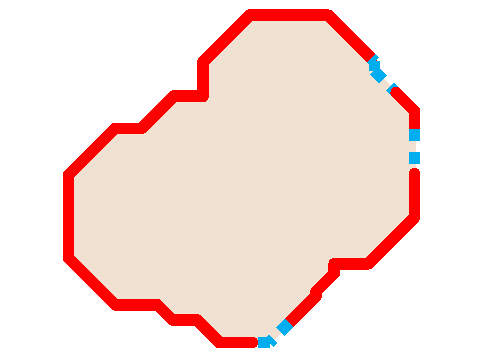
\includegraphics[keepaspectratio, scale=0.4]{./chapters/opg/figures/spmc-example-eps-converted-to.pdf}
    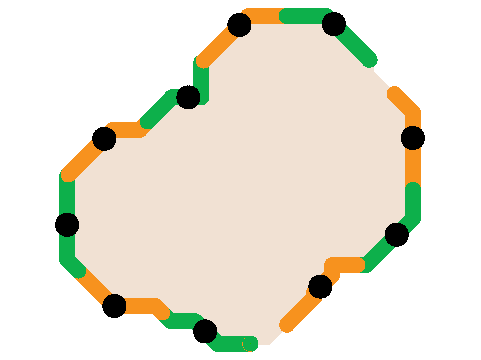
\includegraphics[keepaspectratio, scale=0.4]{./chapters/opg/figures/spmc-solution-eps-converted-to.pdf}
    % \vspace*{-3mm}
    \caption[Example OPG problem instance of SPMC]{\label{fig:opg-spmc-example} 
    An example problem instance when $q = 3$ and $n = 10$. In this case, the 
		optimal cover actually covers one gap.}
    % \vspace*{-4mm}
\end{figure}

\begin{table}[ht!]
    % \vspace*{-3mm}
    \footnotesize
    \centering
    \begin{tabular}{|c|c|c|c|c|c|c|} 
        \hline
        \diagbox{$q$}{$n$}       & $10^1   $ & $10^2   $ & $10^3  $  & $10^4   $ & $10^5$   \\ \hline       
        \rule{0pt}{2.5ex} $10^2$ & $0.013  $ & $0.015  $ & $0.016 $  & $0.016  $ & $0.017$  \\ \hline   
        \rule{0pt}{2.5ex} $10^3$ & $1.363  $ & $1.595  $ & $1.622 $  & $1.634  $ & $1.641$  \\ \hline   
        \rule{0pt}{2.5ex} $10^4$ & $159.404$ & $188.497$ & $210.492$ & $212.473$ & $212.780$\\ \hline   
    \end{tabular}
    \vspace*{-3mm}
    \caption{\label{eval:opg-spmc} \algoSRG~computation time (seconds)}
    \vspace*{-4mm}
\end{table}


%\subsubsection{\algoSRG} 
%To generate a problem of a single perimeter divided by interlaced segments and gaps, 
%we first create an arbitrary polygon $R$. Then, we uniformly randomly sample $2q$ points 
%on $\partial R$ to divide it into $q$ segments and $q$ gaps. 
%An example problem instance along with its optimal cover is shown in 
%~\ref{fig:spmc-example}. The computation time of 
%\algoSRG~under different $q$ and $n$ is presented in Table~\ref{eval:spmc}.

For multiple perimeters containing multiple components, $m$ polygons 
are created with $len(\partial R_i)$ randomly distributed in $[1, 10]$. 
For setting $q_i$, we fix a $q$ and let $q_i = q(0.5 + random(0, 1))$. 
Representative computation results of \algoMRG are listed in 
Table~\ref{eval:opg-mpmc}.
%whose perimeters' lengths are uniformly randomly sampled from interval $(1, 10)$. 
%The computation time under different $m$, $q$, and $n$ values are provided in Table~\ref{eval:mpmc}. 
%We observe that with the same $q$, $n$ parameters, the computation time is directly proportional to $m$.
\begin{table}[ht!]
    \vspace*{-2mm}
    \footnotesize
    \centering
    \begin{tabular}{|c|c|c|c|c|c|c|} 
        \hline
        \multirow{2}{*}{$q$} & \multirow{2}{*}{$n$} & \multicolumn{5}{|c|}{$m$} \\ \cline{3-7}
        \rule{0pt}{2.5ex} & & $10$ & $20$ & $30$ & $40$ & $50$ \\ \hline
        %\rule{0pt}{2.5ex} $10^1$ & $10^2$ & $ 0.015$ & $ 0.027$ & $ 0.039$ & $ 0.045$ & $ 0.054$ \\ \hline
        \rule{0pt}{2.5ex} $10^1$ & $10^3$ & $ 0.047$ & $ 0.063$ & $ 0.076$ & $ 0.091$ & $ 0.108$ \\ \hline
        %\rule{0pt}{2.5ex} $10^2$ & $10^2$ & $ 1.492$ & $ 2.784$ & $ 4.168$ & $ 5.404$ & $ 6.444$ \\ \hline
        \rule{0pt}{2.5ex} $10^2$ & $10^3$ & $ 2.191$ & $ 3.771$ & $ 5.523$ & $ 7.707$ & $ 9.369$ \\ \hline
        \rule{0pt}{2.5ex} $10^2$ & $10^4$ & $ 7.105$ & $ 9.619$ & $11.369$ & $12.760$ & $15.107$ \\ \hline
    \end{tabular}
    \vspace*{-3mm}
    \caption{\label{eval:opg-mpmc} \algoMRG~computation time (seconds)}
    \vspace*{-4mm}
\end{table}

Due to limited space, only selected essential performance data is 
presented here. More complete performance data and associate analysis 
can be found in the Appendix. 


\subsection{Two Applications Scenarios}
\noindent\textbf{Securing a perimeter}. As a first application, consider
a situation where a crime has just been committed at the Edinburgh 
Castle (see ~\ref{fig:opg-edinburgh}). The culprit remains in the confines 
of the castle but is mixed within many guests at the scene. As the 
situation is being investigated and suppose that the brick colored 
buildings are secured, guards (either personnel or a number of drones) may 
be deployed to ensure the culprit does not escape by climbing down the 
castle walls. Using \algoSRG, a deployment plan can be quickly computed 
given the amount of resources at hand so that each guard only needs to 
secure a minimum length along the castle walls. ~\ref{fig:opg-edinburgh} 
shows the optimal deployment plan for $15$ guards. 

\begin{figure}[ht]
	\vspace*{-2mm}
	\begin{center}
		\begin{overpic}[width=0.4\textwidth, tics=5]{./chapters/opg/figures/castle_15.eps}
			% \put(82,44){{\small $\W$}}
		\end{overpic}
	\end{center}
	\vspace*{-4.5mm}
	\caption[Optimal deployment of $15$ guards around walls of the Edinburgh Castle]
	{\label{fig:opg-edinburgh} Optimal deployment of $15$ guards around 
	walls of the Edinburgh Castle. The brick colored structures are buildings 
	that create gaps along the boundary.}
	%\vspace*{-3mm}
\end{figure}

\noindent\textbf{Fire monitoring}. In a second application, consider 
~\ref{fig:opg-forest} where a forest fire has just been put out in 
multiple regions. As there is still some chance that the fire may 
rekindle and spread, for prevention, a team of firefighters is to be 
deployed to watch for the possible spreading of the fire. Here, in 
addition to using \algoMRG to compute optimal locations for deploying 
the firefighters, we also generate minimum time trajectories for the 
firefighters to reach their target locations while avoiding going 
through the dangerous forests. This is done via solving a bottleneck 
assignment problem \cite{burkard1999linear}.
Note that the lake region creates gaps that cannot be traveled by the 
firefighters; this can be handled by making these gaps infinitely large. 
~\ref{fig:opg-forest} shows the optimal locations for $34$ firefighters. 
Animations of the deployment process and other test cases can be found 
in the accompanying video. 

\begin{figure}[ht]
	\vspace*{-2mm}
	\begin{center}
		\begin{overpic}[width=0.7\textwidth,tics=5]{./chapters/opg/figures/forest_solution.eps}
			%\put(82,44){{\small $\W$}}
		\end{overpic}
	\end{center}
	\vspace*{-4.5mm}
	\caption{\label{fig:opg-forest}  Optimal deployment of $34$ firefighters for 
	forest fire rekindling prevention.}
	\vspace*{-3mm}
\end{figure}




\subsection{Conclusion and Discussion}\label{section:opg-conclusion}
In this paper, we propose the \opg problem to model the allocation of 
large robotic swarms to cover complex 1D topological domains with 
optimality guarantees. For all variants under the \opg formulation 
umbrella, we have developed highly efficient algorithms for solving 
\opg exactly. In addition to rigorous proofs backed by formal analysis, 
extensive computational experiments further confirm the effectiveness of 
these algorithms. Moreover, practical relevance of \opg is demonstrated 
through the integration of \opg into realistic task (assignment) and motion 
planning scenarios. 

The study raises many additional interesting open questions; we mention 
a few here. 
%
First, the approach taken in this work is a {\em centralized} one where 
decision is made at the global level. It would be highly interesting to 
explore whether the same can be achieved with {\em decentralized} methods,
which have many advantages. For example, it may be the case that the 
gaps along the boundaries are not known {\em a priori} and must be measured
by the robots. In such cases, a centralized plan can be hard to come by. 
%
Second, as mentioned in Section~\ref{section:opg-problem}, the 
current \opg formulation assumes that the robots are confined to the 
boundaries $\partial \R$, which is one of many possible choices 
in terms of the robots' sensing and/or motion capabilities. In future study,
we plan to examine additional practical robot sensing and motion models. 
%
Third, as exact optimal algorithms are emphasized here, issues including 
uncertainty and robustness have not been touched in the current treatment, 
which are important elements when it comes to the deployment of a robotic 
swarm to tackle real-world challenges. 






\section{Perimeter Guarding with Heterogeneous Defenders}

\def\R{\mathcal R}
\def\C{\mathcal C}
\def\S{\mathcal S}
\def\P{\mathcal P}
\def\G{\mathcal G}
\def\W{\mathcal W}
\def\opg{{\sc {OPG}}\xspace}
\def\opglr{{\sc {OPG${}_{LR}$}}\xspace}
\def\opglrd{{\sc {D-OPG${}_{LR}$}}\xspace}
\def\opgmc{{\sc {OPG${}_{MC}$}}\xspace}

\newcommand{\argmin}[1]{\underset{#1}{\operatorname{arg}\,\operatorname{min}}\;}
\newcommand{\argmax}[1]{\underset{#1}{\operatorname{arg}\,\operatorname{max}}\;}

\def\twopart{\textbf{\textsc{Partition}}\xspace}
\def\tpart{\textbf{\textsc{$3$-Partition}}\xspace}
\def\ttkp{\textbf{\textsc{Knapsack}}\xspace}
\def\ttukp{\textbf{\textsc{Unbounded Knapsack}}\xspace}
\def\ttbp{\textbf{\textsc{Bin Packing}}\xspace}
\def\subsetsum{\textbf{\textsc{Subset Sum}}\xspace}

\subsection{Introduction}\label{sec:opgext-intro}
Consider the scenario where many mobile guards (or sensors) are to be deployed 
to patrol 
the perimeter of some 2D regions (~\ref{fig:opgext-ex}) against intrusion, where 
each guard may effectively cover a continuous segment of a region's boundary. 
When part of a boundary need not be secured, e.g., there may already be 
some existing barriers (the blue segments in ~\ref{fig:opgext-ex}), optimally 
distributing the robots so that each robot's coverage is minimized becomes 
an interesting and non-trivial computational task \cite{fenghangaoyu2019efficient}. 
It is established \cite{fenghangaoyu2019efficient} that, when the guards have 
the same capabilities, the problem, called the {\em optimal perimeter guarding} 
(\opg), resides in the complexity class P (polynomial time class), 
even when the robots must be distributed across many different boundaries. 

\begin{figure}[ht]
\begin{center}
\begin{overpic}[width=0.7\textwidth,tics=5]{chapters/opg-ext/figures/opg-eps-converted-to.pdf}
%\put(26,20){{\small $R_1$}}
%\put(20,39){{\small \textcolor{red}{$P_1$}}}
%\put(66,28){{\small $R_2$}}
%\put(54,40){{\small \textcolor{green}{$P_2$}}}
%\put(82,44){{\small $\W$}}
\end{overpic}
\end{center}
\caption[A scenario where boundaries of three (gray) regions must be secured]
{\label{fig:opgext-ex} A scenario where boundaries of three (gray) 
regions must be secured. Zooming in on part of the boundary of one 
of the regions (the part inside the small circle), portions of the 
boundary (the red segments) must be guarded while the rest (the 
blue dotted segments) does not need guarding. For example, the zoomed-in 
part of the boundary may be monitored by two mobile robots, each patrolling
along one of the green segments.}
\end{figure}

In this work, we investigate a significantly more general version of \opg 
where the mobile guards may be heterogeneous. More specifically, two 
formulations with different guarding/sensing models are addressed in our 
study. 
%
In the first, the number of available robots is fixed where robots of 
different types have a fixed ratio of capability (e.g., one type of 
robot may be able to run faster or may have better sensor). The guarding task 
must be evenly divided among the robots so that each robot, regardless of 
type, will not need to bear a too large coverage/capability ratio. This 
formulation is denoted as {\em optimal perimeter guarding with limited 
resources} or \opglr.
%
In the second, the number of robots is unlimited; instead, for each type, 
the sensing range is fixed with a fixed associated cost. The goal here is 
to find a deployment plan so as to fully cover the perimeter while minimizing 
the total cost. We call this the {\em optimal perimeter guarding with 
minimum cost} problem, or \opgmc. 

Unlike the plain vanilla version of the \opg problem, we establish that both 
\opglr and \opgmc are NP-hard when the number of robot types is part of the 
problem input. They are, however, at different hardness levels. \opglr is shown 
to be NP-hard in the strong sense, thus reducing the likelihood of finding a fully
polynomial time approximation scheme (FPTAS).
% solutions to even approximately solving it to arbitrary precision. 
Nevertheless, for the more practical case where the number of robot types 
is a constant, we show that \opglr can be solved using a pseudo-polynomial 
time algorithm with reasonable scalability. On the other hand, we show that 
\opgmc is weakly NP-hard through the establishment of a pseudo-polynomial 
time algorithm for \opgmc with arbitrary number of robot types. 
We further show that, when the number of robot types is fixed, \opgmc can be 
solved in polynomial time through a fixed-parameter tractable (FPT) approach.
This paragraph also summarizes the main contributions of this work. 

A main motivation behind our study of the \opg formulations is to address 
a key missing element in executing autonomous, scalable, and optimal robot 
deployment tasks. Whereas much research has been devoted to multi-robot 
motion planning \cite{ErdLoz86,arai2002advances} with great success, e.g., 
\cite{van2008reciprocal,smith2009monotonic,ayanian2010decentralized,turpin2014capt,
alonso2015multi,SolYu15}, existing results in the robotics literature appear 
to generally assume that a target robot distribution is already provided; the 
problem of how to effectively generate optimal deployment patterns is largely 
left unaddressed. It should be noted that control-based solutions to the 
multi-agent deployment problem do exist, e.g.,\cite{ando1999distributed,
jadbabaie2003coordination,cortes2004coverage,ren2005consensus,
schwager2009optimal,yu2012rendezvous,morgan2016swarm}, but the final solutions 
are obtained through many local iterations and generally do not come with 
global optimality guarantees. For example, in \cite{cortes2004coverage}, 
Voronoi-based iterative methods compute locally optimal target formations 
for various useful tasks. In contrast, this work, as well as 
\cite{fenghangaoyu2019efficient}, targets the scalable computation of globally optimal 
solutions. 
%To have an end-to-end system, the autonomous generation
%of deployment plan is clearly crucial. Where computational solutions for 
%\cite{alphago}. 
%\jy{Maybe mention alphago?}

As a coverage problem, \opg may be characterized as a 1D version 
of the well-studied Art Gallery problems  \cite{o1987art,shermer1992recent},
which commonly assume a sensing model based on line-of-sight 
visibility\cite{lozano1979algorithm}; the goal is to ensure that every point
in the  interior of a given region is visible to at least one of the deployed 
guards. Depending on the exact formulation, guards may be placed on 
boundaries, corners, or the interior of the region. Not surprisingly, Art
Gallery problems are typically NP-hard \cite{lee1986computational}. Other
than Art Gallery, 2D coverage problems with other sensing models, e.g., 
disc-based, have also been considered \cite{thue1910dichteste,hales2005proof,
drezner1995facility,cortes2004coverage,pavone2009equitable,
pierson2017adapting}, where some formulations prevent the overlapping 
of individual sensing ranges \cite{thue1910dichteste,hales2005proof} while 
others seek to ensure a full coverage which often requires intersection
of sensor ranges. 
%
In viewing of these studies, this study helps painting a broader landscape 
of sensor coverage research.

In terms of structural resemblance, \opglr and \opgmc share many similarities 
with {\em bin packing}  \cite{johnson1973near} and other related problems. 
In a bin packing problem, objects are to be selected to fit within bins of 
given sizes. Viewing the segments (the red ones in ~\ref{fig:opgext-ex}) as 
bins, \opg seeks to place guards so that the segments are fully contained in 
the union of the guards' joint coverage span. In this regard, \opg is a dual
problem to bin packing since the former must overfill the bins and the later 
cannot fully fill the bins. In the extreme, however, both bin packing and 
\opg converge to a \subsetsum \cite{karp1972reducibility} like problem where 
one seeks to partition objects into halves of equal total sizes, i.e., the 
objects should fit exactly within the bins. With an additional cost term, 
\opgmc has further similarities with the \ttkp problem \cite{lueker1975two}, 
which is weakly NP-hard \cite{dantzig1957discrete}.

The rest of the paper is organized as follows. In Section~\ref{sec:opgext-problem},
mathematical formulations of the two \opg variants are fully specified. In
Section~\ref{sec:opgext-hardness}, both \opglr and \opgmc are shown to be 
NP-hard. Despite the hardness hurdles, in Section~\ref{sec:opgext-algorithm}, 
multiple algorithms are derived for \opglr and \opgmc, including effective
implementable solutions for both. In Section~\ref{sec:opgext-application},
we perform numerical evaluation of selected algorithms and demonstrate 
how they may be applied to address multi-robot deployment problems. We 
discuss and conclude our study in Section~\ref{sec:opgext-conclusion}. Please
see \url{https://youtu.be/6gYL0_B3YTk} for an illustration of the problems 
and selected instances/solutions. 

\subsection{Preliminaries}\label{sec:opgext-problem}
Let $\W \subset \mathbb R^2$ be a compact (closed and bounded) 
two-dimensional workspace. There are  $m$ pairwise disjoint {\em 
	regions} $\R = \{R_1, \ldots, R_m\}$ where each region $R_i \subset \W$ 
is homeomorphic to the closed unit disc, i.e., there exists a continuous 
bijection $f_i: R_i \to \{(x, y) \mid x^2 + y^2 \le 1\}$ for all $1 \le 
i \le m$. For a given region $R_i$, let $\partial R_i$ be its (closed) 
boundary (therefore, $f_i$ maps $\partial R_i$ to the unit circle  
$\mathbb S^1$). With a slight abuse of notation, define $\partial \R 
= \{\partial R_1, \ldots, \partial R_m\}$. Let $P_i \subset \partial R_i$ 
be the part of $\partial R_i$ that is accessible, specifially, not blocked by 
obstacles in $\W$. This means that each $P_i$ is either a single closed 
curve or formed by a finite number of (possibly curved) line segments. 
Define  $\P = \{P_1, \ldots, P_m\} \subset \W$ as the {\em perimeter} 
of $\R$ which must be {\em guarded}. More formally, each $P_i$ is 
homeomorphic to a compact subset of the unit circle (i.e., it is 
assumed that the maximal connected components of $P_i$ are closed 
line segments). For a given $P_i$, each one of its maximal connected 
component is called a {\em perimeter segment} or simply a {\em segment}, 
whereas each maximal connected component of $\partial R_i \backslash P_i$ 
is called a {\em perimeter gap} or simply a {\em gap}. An example setting is 
illustrated in Fig.~\ref{fig:example-boundaries} with two regions. 
\definecolor{BrickRed}{RGB}{176, 50, 28}
\definecolor{ForestGreen}{RGB}{0, 155, 85}
\begin{figure}[ht]
	\begin{center}
		\begin{overpic}[width=0.7\textwidth,tics=5]
			{chapters/opg-ext/figures/example-boundaries-eps-converted-to.pdf}
			\put(26,20){{\small $R_1$}}
			\put(20,39){{\small \textcolor{BrickRed}{$P_1$}}}
			\put(66,28){{\small $R_2$}}
			\put(54,40){{\small \textcolor{ForestGreen}{$P_2$}}}
			%\put(79.6,18){{\small $h$}}
			\put(82,44){{\small $\W$}}
		\end{overpic}
	\end{center}
	\caption{\label{fig:example-boundaries} An example of a workspace $\W$ 
		with two regions $\{R_1, R_2\}$. Due to three {\em gaps} on $\partial R_1$, 
		marked as dotted lines within long rectangles, $P_1 \subset \partial R_1$ 
		has three {\em segments} (or maximal connected components); $P_2 = \partial 
		R_2$ has a single segment with no gap.}
\end{figure}

After deployment, some number of robots are to {\em cover} the perimeter 
$\P$ such that a robot $j$ is assigned a continuous closed subset $C_j$ 
of some $\partial R_i, 1 \le i \le m$. All of $\P$ must be {\em covered} 
by $\C$, i.e., 
%
$\bigcup_{P_i \in \P} P_i  \subset \bigcup_{C_j \in \C} C_j$,
%
which implies that elements of $\C$ need not intersect on their interiors. 
Hence, it is assumed that any two elements of $\C$ may share at most their 
endpoints. Such a $\C$ is called a {\em cover} of $\P$. Given a cover 
$\C$, for a $C_j \in \C$, let $len(C_j)$ denote its length (more formally, 
measure). 

To model heterogeneity of the robots, two models are explored in this
study. In either model, there are $t$ types of robots. In the first model,
the number of robots of each type is fixed to be $n_1, \ldots, n_t$ with 
$n = n_1 + \cdots + n_t$. For a robot $1 \le j \le n$, let $\tau_j$ denote 
its type. Each $1 \le \tau \le t$ type of robots has some 
level of {\em capability} or {\em ability} $a_{\tau} \in \mathbb Z^+$. We 
wish to balance the load among all robots based on their capabilities, 
i.e., the goal is to find cover $\C$ for all robots such that the quantity 
\[
\max_{C_j \in \C} \frac{len(C_j)}{a_{\tau_j}},
\]
which represents the largest coverage-capacity ratio, is minimized. 
We note that when all capacities are the same, e.g., $a_{\tau} = 1$ for 
all robots, this becomes the standard \opg problem studied in \cite{FenHanGaoYu19RSS}. 
We call this version of the perimeter guarding problem {\em optimal 
	perimeter guarding with limited resources} or \opglr. The formal 
definition is as follows.

\begin{problem}[Optimal Perimeter Guarding with Limited Resources 
	(\opglr)] Let there be $t$ types of robots. For each type $1\le \tau 
	\le t$, there are $n_{\tau}$ such robots, each having the same 
	capability parameter $a_{\tau}$. Let $n = n_1 + \cdots + n_t$. 
	Given the perimeter set $\P = \{P_1, \ldots, P_m\}$ of a set of 
	2D regions $\R =\{R_1, \ldots, R_m\}$, find a set of $n$ continuous 
	line segments $\C^* = \{C_1^*, \ldots, C_n^*\}$ such that $\C^*$ covers 
	$\P$, i.e., \begin{align}\label{eq:coverage}
	\bigcup_{P_i \in \P} P_i  \subset \bigcup_{C_j^* \in \C^*} C_j^*,
	\end{align}
	such that a $C_j^*$ is covered by robot $j$ of type $\tau_j$, and such that,
	among all covers $\C$ satisfying~\eqref{eq:coverage}, 
	\begin{align}\label{eq:objective}
	\C^* = \underset{\C}{\mathrm{argmin}} \max_{C_j \in \C} 
	\frac{len(C_j)}{a_{\tau_j}}.
	\end{align}
\end{problem}

Whereas the first model caps the number of robots, the second
model fixes the maximum coverage of each type of robot. That is, for 
each robot type $1 \le \tau \le t$, $n_{\tau}$, the number of robots of type $\tau$,
is unlimited as long as it is non-negative, but each such robot can only cover 
a maximum length of $\ell_{\tau}$. 
At the same time, using each such robot incurs a cost of $c_{\tau}$. The 
goal here is to guard the perimeters with the minimum total cost. We 
denote this problem {\em optimal perimeter guarding with minimum 
	cost} or \opgmc. 

\begin{problem}[Optimal Perimeter Guarding with Minimum Cost
	(\opgmc)] Let there be $t$ types of robots of unlimited quantities. 
	For each robot of type $1\le \tau \le t$, it can guard a length of 
	$\ell_{\tau}\in\mathbb{Z^+}$ with a cost of $c_{\tau}\in\mathbb{Z^+}$. Given the perimeter set
	$\P = \{P_1, \ldots, P_m\}$ of a set of 2D regions $\R =\{R_1, \ldots, 
	R_m\}$, find a set of $n = n_1 + \cdots + n_t$ continuous line segments 
	$\C^* = \{C_1^*, \ldots, C_n^*\}$ where $n_{\tau}$ such segments are 
	guarded by type $\tau$ robots, such that $\C^*$ covers $\P$, i.e., 
	\begin{align}\label{eq:coverage2}
	\bigcup_{P_i \in \P} P_i  \subset \bigcup_{C_j^* \in \C^*} C_j^*,
	\end{align}
	such that a $C_j^*$ is covered by robot $j$ of type $\tau_j$, i.e., 
	$C_j^* \le \ell_{\tau_j}$, and such that,
	among all covers $\C$ satisfying~\eqref{eq:coverage2}, 
	\begin{align}\label{eq:objective2}
	\C^* = \underset{\C}{\mathrm{argmin}} \sum_{1 \le \tau \le t} 
	n_{\tau}c_{\tau}.
	\end{align}
\end{problem}


\subsection{Computational Complexity for Variable Number of Robot Types}\label{sec:opgext-hardness}
We explore in this section the computational complexity of \opglr 
and \opgmc. Both problems are shown to be NP-hard with \opglr 
being strongly NP-hard. We later confirm that \opgmc is weakly 
NP-hard (in Section~\ref{sec:algorithm}).

\subsection{Strong NP-hardness of \opglr}\label{subsec:opglr-hardness}
When the number of types $t$ is a variable, i.e., $t$ is not a constant
and may be arbitrarily large,
% (but bounded by $n$), 
\opglr is shown to be NP-hard via the reduction from \tpart \cite{garey1975complexity}:

\vspace*{1mm}
\noindent
PROBLEM: \tpart\\
INSTANCE: A finite set A of $3m$ elements, a bound $B\in \mathbb{Z^+}$, 
% $S$ with $|S| = 3m$,
and a ``size'' $s(a)\in \mathbb{Z^+}$ for each $a\in A$,
such that each $s(a)$ satisfies $B/4 < s(a) <B/2$ and $\sum_{a\in A} s(a) = mB$.\\
QUESTION: Is there a partition of $S$ into $m$ disjoint subsets $S_1, 
\ldots, S_m$ such that for $1\leq i\leq m$, 
$\sum_{a\in S_i} s(a) = B$?
\vspace*{1mm}

%In a \tpart instance, let $\sum_{s \in S} s = B$ and for all $b \in B$, 
%$1/4 < b <  1/2$. Under such conditions, \tpart remains strongly 
%NP-hard \cite{garey1979computer}. We will use this version of the \tpart problem. We mention here that we use fractional values for 
%the elements of $B$ to avoid adding additional variables; this is fine 
%as long as we restrict the involved numbers to be rationals. 
\tpart is shown to be NP-complete in the strong sense\cite{GarJoh79}, 
i.e., it is NP-complete even when all numeric inputs are bounded by a polynomial 
of the input size. 

For the reduction, it is more convenient to work with a decision 
version of the \opglr problem, denoted as \opglrd. In the \opglrd 
problem, $a_{\tau}$ is the actual length robot type $\tau$ covers. 
That is, the coverage length of a robot is fixed. The \opglrd problem 
is specified as follows. 

\vspace*{1mm}
\noindent
PROBLEM: \opglrd\\
INSTANCE: $t$ types of robots where there are $n_{\tau}$ robots for 
each type $1 \le \tau \le t$; $n = n_1 + \cdots + n_t$. A robot of 
type $\tau$ has a coverage capacity $a_{\tau}$. A set of perimeters 
$\P = \{P_1, \ldots, P_m\}$ of a set of 2D regions 
$\R =\{R_1, \ldots, R_m\}$.\\ 
QUESTION: Is there a deployment of $n$ disjoint subsets $C_1, \ldots, C_n$
of $\{\partial R_1, \ldots, \partial R_m\}$ such that 
$P_1 \cup \ldots \cup P_m \subset C_1 \cup \ldots \cup C_n$, where
$C_j$ is a continuous segment for all $1 \le j \le n$, and for each 
$1 \le j \le n$, there is a unique robot whose type $\tau$, $1 \le \tau 
\le t$ satisfies $a_{\tau} \ge len(C_j)$?
\vspace*{1mm}

\begin{theorem}\label{t:opglr-hard}
	\opglr is strongly NP-hard. 
\end{theorem}
\begin{proof}
	A polynomial reduction from \tpart to \opglrd is constructed
	by a restriction of \opglrd. Given a \tpart instance with former notations,
	we apply several restrictions on \opglrd: {\em (i)} there are $3m$ types of robot
	and there is a single robot 
	for each type, i.e., $n_{\tau} = 1$ for $1 \le \tau \le t$, so $n=t=3m$ 
	{\em (ii)} the $3m$ capacities $a_1, \ldots, a_{3m}$ are set to be equal to
	$s(a)$ for each of the $3m$ elements $a\in A$, and {\em (iii)} 
	there are $3m$ perimeters and each perimeter $P_i$ is continuous and
	$len(P_i)=B$ for all $1 \le i \le m$.

	% \begin{comment}
	% In this proof, we work with a further restriction of \opglrd: {\em (i)}
	% there is a single robot for each type, i.e., $n_{\tau} = 1$ for $1 
	% \le \tau \le t$, and {\em (ii)} each perimeter $P_i$ is continuous and
	% %$len(P_i)$ is the same for all $1 \le i \le m$.
	
	% $len(P_i) = B$ for all $1 \le i \le m$.
	% Given a \tpart instance with $\sum_{b_i \in B} b = q$ and $1/4 \le b 
	% \le  1/2$ for all $b_i \in B$, let the corresponding \opglrd instance 
	% have $q$ perimeters, each with a single segment with the same length 
	% $L$. Let there be $3q$ robots, each with a type $1 \le \tau \le 3q$ 
	% and capability parameter $a_{\tau} = b_{\tau} \in B$. The restricted
	% \opglrd problem instance asks a question similar to the \tpart problem: 
	% is there a partition of the robots such that each perimeter of length 
	% $1$ is covered by three robots (notice that it is impossible to reach 
	% a total capacity of $1$ with fewer or more than $3$ robots)? 
	% \end{comment}

	% \begin{comment}
	% We make some rudimentary observations regarding the \opglrd instance 
	% and the related \opglr instance. Since all $q$ perimeters are of length 
	% $L$ each and the total capability of the robots is $q$, the objective 
	% \eqref{eq:objective} cannot be lower than $\frac{qL}{q} = L$, which is 
	% achieved only when each perimeter is covered by robots with total 
	% capability parameter of $1$. Then, because of the requirement $1/4 < 
	% a_{\tau} < 1/2$, if the best possible solution to the related \opglr 
	% instance is to be realized, each perimeter must be covered by exactly 
	% three robots; otherwise, the total capability cannot sum up to $1$. 
	% \end{comment}
	
	With the setup, the reduction proof is straightforward. Clearly, the 
	\tpart instance admits a partition of $A$ into $S_1, \ldots, 
	S_m$ such that $\sum_{a \in S_i} s(a) = B$ for all $1\leq i\leq m$ 
	if and only if a
	valid depolyment exists in the corresponding \opglrd instance. 
	It is clear that the reduction from \tpart to 
	\opglrd is polynomial (in fact, linear). Based on the 
	reduction and because \tpart is strongly NP-hard, so is \opglrd 
	%(by Lemma 4.1 of \cite{garey1975complexity}) 
	and \opglr.
\end{proof}

\begin{remark}
	One may also reduce weakly NP-hard problems, e.g., \twopart
	\cite{karp1972reducibility}, to \opglr for variable number of robot 
	types $t$. Being strongly NP-hard, \opglr is unlikely to admit pseudo-polynomial 
	time solutions for variable $t$. This contrasts with a later result 
	which provides a pseudo-polynomial time algorithm for \opglr for 
	constant $t$, as one might expect in practice where robots have limited 
	number of types. We also note that Theorem~\ref{t:opglr-hard} continues 
	to hold for a single perimeter with multiple segments, each 
	having a length $B$ in previous notation, separated by ``long'' gaps. Obviously, 
	\opglrd is in NP, thus rendering it NP-complete. 
\end{remark}

\subsection{NP-hardness of \opgmc}
The minimum cost \opg variant, \opgmc, is also NP-hard, which may be 
established through reduction from the \subsetsum problem 
\cite{karp1972reducibility}:

\vspace*{1mm}
\noindent
PROBLEM: \subsetsum \\
INSTANCE: A set $B$ with $|B| = n$ and a weight function $w: B \to 
\mathbb Z^+$, and an integer $W$.\\ 
QUESTION: Is there a subset $B' \subseteq B$ such that $\sum_{b \in B'} 
w(b) = W$?
\vspace*{1mm}

\begin{theorem}\label{t:opgmc-hard}
	\opgmc is NP-hard. 
\end{theorem}
\begin{proof}
	Given a \subsetsum instance, we construct an \opgmc instance with a 
	single perimeter containing a single segment with length $L$ to be 
	specified shortly. Let there be $t=2n$ types of robots. For $1 \le i 
	\le n$, let robot type $2i-1$ have $\ell_{2i-1} = c_{2i-1} = 
	w(b_i) + (2^{n + 1} + 2^i)W'$ and let robot type $2i$ have $\ell_{2i} 
	= c_{2i} = (2^{n + 1} + 2^i)W'$. Here, $W'$ can be any integer number no less than 
	$\sum_{b\in B} w(b)$. Set $L = W + (n2^{n+1} + 2^n + \ldots 
	+ 2^1)W'$. We ask the ``yes'' or ``no' decision question of whether there 
	are robots that can be allocated to have a total cost no more than $L$ 
	(equivalently, equal to $L$, as the cost density $c_\tau/l_\tau$
	is always $1$).
	
	Suppose the \subsetsum instance has a yes answer that uses a subset
	$B' \subseteq B$. Then, the \opgmc instance has a solution with cost $L$ 
	that can be constructed as follows. For each $1 \le i \le n$, a single 
	robot of type $2i - 1$ is taken if $b_i \in B'$. Otherwise, a single 
	robot of type $2i$ is taken. This allocation of robots yields a total 
	length and cost of $L$. 
	
	For the other direction, we first show that if the \opgmc instance 
	is to be satisfied, it can only use a single robot from type $2i-1$ 
	or $2i$ for all $1 \le i \le n$. First, if more than $n$ robots are 
	used, then the total cost exceeds $(n + 1)2^{n+1}W' > L$ as $W\leq W'$.
	% because $W' + (2^n + \ldots + 2)W' < 2^{n+1}W'$. 
	Similarly, if less than $n$ 
	robots are used, the total length is at most 
	$(n-1)2^{n+1}W'+(2^{n+1}-1)W'+ W' < L$. 
	Also, to match the $(2^n + \ldots + 2)W'$ part of the cost, exactly one robot 
	from type $2i-1$ or $2i$ for all $1 \le i \le n$ must be taken. 
	Now, if the \opgmc decision instance has a yes answer, if a robot 
	of type $2i -1$ is used, let $b_i \in B$ be part of $B'$, which 
	constructs a $B'$ that gives a yes answer to the \subsetsum instance.
\end{proof}
% add this citation because the proof the hardness probably comes from it
\begin{remark}
	It is also clear that the decision version of the \opgmc problem is 
	NP-complete. The \subsetsum is a weakly NP-hard problem that admits 
	a pseudo-polynomial time algorithm \cite{dantzig1957discrete}. 
	As it turns out, \opgmc, which shares similarities with \subsetsum
	and \ttkp (in particular, \ttukp \cite{ukphardness}), though NP-hard, 
	does admit a pseudo-polynomial time algorithm as well. 
\end{remark}

\begin{comment}
In concluding the section, we note that we have not determined the 
hardness for the case with constant number of robot types. There are 
some recent evidence that such problems may not be as hard as when 
the number of robot types is a fixed input parameter 
\cite{goemans2014polynomiality}.
\end{comment}



\subsection{Exact Algorithms for \opglr and \opgmc}\label{sec:opgext-algorithm}
In this section, we describe three exact algorithms for solving the two 
variations of the \opg problem. First, we present a pseudo-polynomial time
algorithm for \opglr when the number of robot types, $t$, is a fixed constant. 
Given that \opglr is strongly NP-hard, this is in a sense a best possible 
solution. 
%
For \opgmc, in addition to providing a pseudo-polynomial algorithm for 
arbitrary $t$, which confirms that \opgmc is weakly NP-hard, we also provide
a polynomial time approximation scheme (PTAS). We then further show the 
possibility of solving \opgmc in polynomial time when $t$ is a fixed constant. 
We mention that our development in this section focuses on the single 
perimeter case, i.e., $m = 1$, as the generalization to arbitrary $m$ is 
straightforward using techniques described in \cite{fenghangaoyu2019efficient}. With this in mind, 
we also provide the running times for the general setting with arbitrary $m$ 
but refer the readers to \cite{fenghangaoyu2019efficient} on how these running times can be derived. 

For presenting the analysis and results, for the a perimeter $P$ that we work 
with, assume that it has $q$ perimeter segments $S_1, \ldots, S_q$ that need 
to be guarded; these segments are separated by $q$ gaps $G_1, \ldots, G_q$. 
For $1 \le i, i' \le q$, define $S_{i\sim i'} = S_i \cup G_i \cup S_{i+1} \cup \ldots 
\cup G_{i'-1} \cup S_{i'}$ where $i'$ may be smaller than $i$ (i.e., $S_{i\sim i'}$
may wrap around $G_q$),
For the general case with $m$ perimeters, assume that a perimeter $P_i$ has
$q_i$ segments. 
\begin{comment}
\jy{A paper, or anything with some level of complexity to digest, should be 
hierarchical. So, at the beginning of a section, it is good to explain a bit 
of what will be covered so a reader will have an idea of the structure of 
the section.}
\end{comment}

\subsection{Pseudo-Polynomial Time Algorithm for \opglr with Fixed Number
of Robot Types}
\SetKw{Continue}{continue}
\SetKw{True}{true}
\SetKw{False}{false}
\SetKwComment{Comment}{\%}{}
\SetKwInOut{Input}{Input}
\SetKwInOut{Output}{Output}
\def\inc{{\sc Inc}\xspace}
\def\knapsack{\textbf{\textsc{Knapsack}}\xspace}
\def\opglrfeasible{{\sc OPG-lr-Feasible}\xspace}
\def\opgmcdp{{\sc OPG-mc-DP}\xspace}
We set to develop an algorithm for \opglr for arbitrary $t$, the number of robot 
types; the algorithm runs in pseudo-polynomial time when $t$ is a constant. 
At a higher level, our proposed algorithm works as follows. First, our main effort 
here goes into deriving a feasibility test for \opglrd as defined in 
Section~\ref{subsec:opgext-opglr-hardness}. With such a feasibility test, we can then 
find the optimal $\frac{len(C_j)}{a_{\tau_j}}$ in \eqref{eq:opgext-opg-objective} via binary search.
Let us denote the optimal value of $\frac{len(C_j)}{a_{\tau_j}}$ as $\ell^*$. 

\subsubsection{Feasibility Test for \opglrd} The feasibility test for \opglrd 
essentially tries different candidate $\ell$ to find $\ell^*$. Our implementation uses 
ideas similar to the pseudo-polynomial time algorithm for the \knapsack problem which
is based on dynamic programming (DP). In the test, we work with a fixed starting point on 
$P$, which is set to be the counterclockwise end point of a segment $S_i$, $1 \le i \le q$. 
Essentially, we maintain a $t$ dimensional array $M$ where dimension $\tau$
has a size of $n_{\tau} +1$. An element of the array, $M[n_1']\ldots[n_t']$, holds the 
maximal distance starting from $S_i$ that can be covered by $n_1'$ type 1 robots, 
$n_2'$ type 2 robots, and so on. The DP procedure \opglrfeasible($i, \ell$), outlined in 
Algorithm~\ref{algo:opgext-opglrd}, incrementally builds this array $M$. For convenience,
in the pseudo code, $M[\vec{x}]$ denotes an element of $M$ with $\vec{x}$ being 
a $t$ dimensional integer vector. 

\begin{algorithm}
	\DontPrintSemicolon
	% \KwData{$n_1, n_2, \cdots, n_k$ robots, $l_1, l_2, \cdots, l_n$ coverage distance}
	\KwData{$n_1, \ldots, n_t$, $a_1, \ldots, a_t$,
		$S_1, \ldots, S_q$, $G_1, \ldots, G_q$}
	\KwResult{\True or \False,  indicating whether $S_1, \ldots, S_q$ can be covered}
	%\Begin{
		Initialize $M$ as a $t$ dimensional array with dimension $\tau$ having a size of $n_{\tau} + 1$;\;
		$\ell_{\tau} \leftarrow a_{\tau}\ell$ for all $1\le \tau \le t$;\;
		\For{$ \vec{x} \in [0, n_1]\times\dots\times[0,n_t]$}{
            $M[\vec{x}]\leftarrow 0$;\;
			\For{$j = 1$ \KwTo $t$}{
				\lIf{$\vec{x}_j = 0$}{\Continue;}
				$\vec{x'}\leftarrow\vec{x}$; $\vec{x'}_j \leftarrow \vec{x'}_j - 1$;\;
				$M[\vec{x}]\leftarrow max$($M[\vec{x}]$, \inc($M[\vec{x'}], \ell_j$));\;
			}
			% \For{$i_2 \leftarrow 1$ \KwTo $n_2$}{
			% $\cdots$\;
			% \For{$i_k \leftarrow 1$ \KwTo $n_k$}{
			% $DP[i_1][i_2]\cdots[i_k]\leftarrow$ min(Increment($DP[i_1-1][i_2]\dots[i_k],\cdots,l_1$), Increment($DP[i_1][i_2-1]\dots[i_k], l_2$), $\cdots$, Increment($DP[i_1][i_2]\cdots[i_k-1],l_k$)\;
			% }
			% }
		}
		\Return{$M[n_1]\ldots[n_t] \ge len(S_{i\sim {i-1}})$};
	%}
	\caption{\opglrfeasible($i, \ell$)}\label{algo:opgext-opglrd}
\end{algorithm}

In Algorithm~\ref{algo:opgext-opglrd}, the procedure \inc($L, \ell$) checks how much of the 
perimeter $P$ can be covered when an additional coverage length $\ell$ is added, 
assuming that a distance of $L$ (starting from some $S_i$) is already covered. An 
illustration of how \inc($L, \ell$) works is given in ~\ref{fig:opgext-inc}.
 

\begin{figure}[ht]
	\begin{center}
		\begin{overpic}[width=0.7\textwidth,tics=5]
			{chapters/opg-ext/figures/inc-eps-converted-to.pdf}
			\put(26,10){{\small $L$}}
			\put(61,10){{\small $\ell$}}
			\put(30,1){{\small \textsc{Inc}($L$, $\ell$)}}
		\end{overpic}
	\end{center}
    \caption[Illustration of a solution]{\label{fig:opgext-inc}Suppose starting from the fixed left point, a 
		length of $L$ on the boundary is successfully guarded by a group of 
		robots. Then, a robot with coverage capacity $\ell$ is appended to 
		the end of the group of robots to increase the total guarded distance. 
		In the figure, the added additional capacity $\ell$ can fully cover 
		the third red segment plus part of the third (dashed) gap. Because 
		there is no need to cover the rest of the third gap, 
		\textsc{Inc}($L$, $\ell$) extends to the end of the gap.}
\end{figure}

%Denote procedure $Inc(L, \ell)$ as the length of boundary successfully guarded from $L$ using a continuous segment length of $\ell$.

%It is straightforward to see that Algorithm~\ref{algo:opglrd} has a running 
%time of $O(t\Pi_{i=1}^{t} (n_i+1))$ if we populate $M$ gradually.

By simple counting, the complexity of the algorithm is
$O(q\cdot t\cdot\Pi_{\tau=1}^{t} (n_{\tau}+1))$. However, the amortized
complexity of \inc($\cdot$) for each $\tau$ is $O(q+n_{\tau})$; the algorithm thus 
runs in $O(t\cdot\Pi_{{\tau}=1}^{t}(n_{\tau}+1)+q\cdot\sum_{{\tau}=1}^{t} 
\Pi_{{\tau'}\neq {\tau}} (n_{\tau'} +1))$, 
which is pseudo-polynomial for fixed $t$. After trying every possible starting 
position $i$ with \opglrfeasible($i, \ell$), for a fixed candidate $\ell$, 
\opglrd is solved in $O(q \cdot t\cdot\Pi_{{\tau}=1}^{t}(n_{\tau}+1) + 
q^2\cdot\sum_{{\tau}=1}^{t} \Pi_{{\tau'}\neq {\tau}} (n_{\tau'} +1))$.

\subsubsection{Solving \opglr using Feasibility Test for \opglrd}
Using \opglrfeasible($i, \ell$) as a subroutine to check feasibility for a given $\ell$, 
bisection can be applied over candidate $\ell$ to obtain $\ell^*$. For completing 
the algorithm, one needs to establish when the bisection will stop (notice that, 
even though we assume that $a_\tau \in \mathbb{Z^+}$, for each $1\leq \tau \leq t$, $\ell^*$ need not be 
an integer). 

To derive the stop criterion, we note that given the optimal $\ell^*$, there must 
exist some $S_{i\sim i'}$ that is ``exactly'' spanned by the allocated robots.
That is, assume that $S_{i\sim i'}$ is covered by $n_1'$ of type $1$ robots
and $n_2'$ of type $2$ robots, and so on, then 
\begin{align}\label{eq:opgext-exact}
\ell^* = \frac{len(S_{i\sim i'})}{\sum_{1 \le \tau \le t} a_{\tau}\cdot n_{\tau}'}.
\end{align}

\eqref{eq:opgext-exact} must hold for some $S_{i\sim i'}$ because if not, the solution 
is not tight and can be further improved. Therefore, the bisection process for 
locating $\ell^*$ does not need to go on further after reaching a certain granularity\cite{fenghangaoyu2019efficient}.
%$1/\sum_{1 \le \tau \le t} a_{\tau}\cdot n_{\tau}$. 
With this established, using 
similar techniques from \cite{fenghangaoyu2019efficient} (we omit the technical detail as it is quite 
complex but without additional new ideas beyond beside what is already covered 
in \cite{fenghangaoyu2019efficient}), we could prove that the full algorithm needs 
no more than $O(q\log(\sum_{\tau}n_{\tau}+q)$ calls to \opglrfeasible($i, \ell$).
%$O(t\Pi_{i=1}^{t}(n_i+1)+q\sum_{i=1}^{t} \Pi_{j\neq i} (n_j +1))$
This directly implies that \opglr also admits a pseudo-polynomial algorithm for fixed $t$.
% \sw{The complexity here is the decision version of single perimeters}
\subsubsection{Multiple Perimeters}
Also using techniques developed in \cite{fenghangaoyu2019efficient}, the single perimeter 
result can be readily generalized to multiple perimeters. We omit the mechanical
details of the derivation and point out that the computational complexity in this case becomes
$\tilde{O}( (m-1)\cdot((\Pi_{\tau=1}^t n_\tau) / \max_\tau n_\tau)^2 + 
\sum_{k=1}^{m} (t\cdot q_k\cdot \Pi_{{\tau}=1}^{t}(n_{\tau}+1)+
q_k^2\sum_{{\tau}=1}^{t} \Pi_{{\tau'}\neq {\tau}} (n_{\tau'} +1)))$.
% \sw{the complexity here is for decision version of multiple perimeters, starting
%  from a specific starting point}
%\jy{I updated the formula as it seems to be wrong. Also changed $r$ to $m$.}

\subsection{Polynomial Time Algorithm for \opgmc with Fixed Number of Robot Types}
%\subsection{$OPG_{MC}$}
The solution to \opgmc will be discussed here. A method based on DP 
will be provided first, which leads to a polynomial time algorithm for a 
fixed number of robot types and a pseudo-polynomial time algorithm when the number 
of robot types is not fixed. For the latter case, a polynomial time approximation 
scheme (PTAS) will also be briefly described.
\subsubsection{Dynamic Programming Procedure for \opgmc}
\def\sol{{\sc Sol}}
\def\presol{{\sc PreSolve}}
When no gaps exist, the optimization problem becomes a covering 
problem as follows. Let $c_{\tau}$, $\ell_{\tau}$, $n_{\tau}$ correspond to the cost, 
coverage length, and quantity of robot type ${\tau}$, respectively, and let total 
length to cover be $L$. We are to solve the optimization problem
\begin{align}\label{eq:opgext-ip}
    \min \sum_{\tau} c_{\tau} \cdot n_{\tau} \quad s.t.\, \quad
    \sum_{\tau} \ell_{\tau} \cdot n_{\tau} \geq L, n_{\tau}\geq 0.
\end{align}

Let the solution to the above integer programming problem be \sol($L$).
Notice that, for $S_{i\sim i'}:=\{S_i,\ G_i, \dots, 
G_{i'-1}, S_{i'}\}$, the minimum cost cover is by either: {\em (i)} 
covering the total boundary without skipping any gaps, 
%
or {\em (ii)} skipping or partially covering some gap, for example $G_k, 
i \le k \le j-1$.
%
In the first case, the minimum cost is exactly \sol$(\lceil len(S_{i\sim(i+k)}\rceil)$.
%
In the second case, the optimal structure for the two subsets of perimeter 
segments $S_{i\sim k}$ and $S_{(k+1)\sim j}$ still holds. This means that the 
continuous perimeter segments $S_{i\sim j}$ can be divided into two parts, 
each of which can be treated separately. This leads to a DP approach for \opgmc.
With $M[i][j]$ denoting the minimum cost to cover $S_{i\sim j}$, the DP recursion 
is given by
\[
	\scalebox{0.93}{$M[i][j] = \min(\textit{\sol}(\lceil len(S_{i\sim j})\rceil), \displaystyle\min_k(M[i][k]+M[k+1][j]))$}
\]

The DP procedure is outlined in Algorithm~\ref{alg:opgext-opgmc}. In the pseudo code, 
it is assumed that indices of $M$ are modulo $q$, e.g., $M[2][q+1] 
\equiv M[2][1]$. $tmp$ is a temporary variable. 
\begin{comment}
\jy{Generally mathematicians and theoretical computer scientists use 
	$\ell_1, \ldots, \ell_t$ instead of $\ell_1, \ell_2, \ldots, \ell_t$. The later is more 
	redundant. Also, normally we use ldots instead of cdots. I changed $C$ to $M$ since 
    $C$ is used elsewhere. I changed $==$ to $=$ to save space.}
\end{comment}
\begin{algorithm}
    \DontPrintSemicolon
    % \KwData{$n_1, n_2, \cdots, n_k$ robots, $l_1, l_2, \cdots, l_n$ coverage distance}
    \KwData{$\ell_1, \dots, \ell_t$, $c_1, \ldots, c_t$,
    	$S_1, \ldots, S_q$, $G_1, \ldots, G_q$}
    \KwResult{$c^*$, the minimum covering cost}
   %\Begin{
    $M \leftarrow$ a $q\times q$ matrix; $c^* \leftarrow \infty$; \;
    \For{$k \leftarrow 0$ \KwTo $q-1$}{
        \For{$i\leftarrow 1 $ \KwTo $q$}{
            $tmp \leftarrow\ $\sol$(\lceil len(S_{i\sim(i+k)}) \rceil)$; \;
            \For{$j\leftarrow i$ \KwTo $i+k-1$}{
                $tmp \leftarrow \min(tmp, M[i][j] + M[j+1][i+k])$;
            }
            $M[i][i+k] \leftarrow c$;\;
            \lIf{$k = q-1$}{$c^* \leftarrow \min(c^*, M[i][i+k])$;}
        }
    }
    \Return{$c^*;$}
    %}
    \caption{\opgmcdp}
    \label{alg:opgext-opgmc}
\end{algorithm}

\subsubsection{A Polynomial Time Algorithm for \opgmc for a Fixed Number of Robot Types}
We mention briefly that, by a result of Lenstra \cite{lenstra1983integer}, the optimization problem 
~\eqref{eq:opgext-ip} is in P (i.e., polynomial time) when $t$ is a constant. The running time of 
the algorithm \cite{lenstra1983integer} is however exponential in $t$. 

\subsubsection{A Pseudo-polynomial Time Algorithm for Arbitrary $t$}
As demonstrated in the hardness proof, similarities exist between \opg and the \knapsack 
problem. The connection actually allows the derivation of a pseudo-polynomial time algorithm
for arbitrary $t$. To achieve this, we use a routine to pre-compute \sol($L$), called 
\presol(), which is itself a DP procedure similar to that for the \knapsack problem. The 
pseudo code of \presol() is given in Algorithm~\ref{algo:opgext-presol}.
\presol() runs in time $O(t\cdot\lceil len(\partial R)\rceil))$. Overall, 
Algorithm~\ref{alg:opgext-opgmc} then runs in time $O(q^3+t\cdot\lceil len(\partial R\rceil))$.
%\jy{Is this running time correct?}

\begin{algorithm}
	\DontPrintSemicolon
	\KwData{$\ell_1, \ldots, \ell_t$, $c_1, \ldots, c_t$}
	\KwResult{A lookup table for retrieving \sol($L$)}
	%\Begin{
		$I_{max} = \lceil len(\partial R)\rceil$; \Comment{\small $I_{max}$ is an integer.}
		$M' \leftarrow$ an array of length $I_{max} + 1$; 
		$M'[0]\leftarrow 0$;\;
		\For{$L \leftarrow$ $1$ \KwTo $I_{max}$}{
			$M'[L]\leftarrow \infty$; \;
			\For{${\tau}\leftarrow 1$ \KwTo $t$}{
				$tmp \leftarrow (L<\ell_{\tau}\ ?\ 0\ :\ M'[L-\ell_{\tau}]) + c_{\tau}$;\;
				$M'[L] \leftarrow min(M'[L], tmp)$;\;
			}
		}
		\Return{$M'$}
	%}
	\caption{{\sc PreSolve}}\label{algo:opgext-presol}
\end{algorithm}

%After the preprocessing, 
%the Solution(L) is just an access of $Sol[L]$. 
%Algorithm \ref{alg:opgmc} still applies and the only modification is a simple replacement of 
%\sol($L$) with $Sola[L]$. This make the complexity of \ref{alg:opgmc} drop to $O(q^3)$.
% \begin{algorithm}
%     \DontPrintSemicolon
%     % \KwData{$n_1, n_2, \cdots, n_k$ robots, $l_1, l_2, \cdots, l_n$ coverage distance}
%     \KwData{$l_1, l_2, \cdots, l_k$ coverage distance, $c_1, c_2,\cdots,c_k$ deployment cost}
%     \KwResult{Minimum cost for covering the perimeter}
%     \Begin{
%     $DP \leftarrow$ 1-D array length of L with data initialized to $\infty$\;
%     $DP[0]\leftarrow 0 $\;
%     $Result\leftarrow \infty$\;
%     \For{$l \leftarrow 0$ \KwTo $L$}{
%     \If{$DP[l] = \infty$}{  \Continue\;}
%     \For{$i \leftarrow 1$ \KwTo $k$}{
%     $nextEnd \leftarrow $Increment($l, l_i$)\;
%     $DP[nextEnd] = \min(DP[nextEnd], DP[l]+c_i)$\;
%     \If{$nextEnd\geq L$}{Result$\leftarrow \min(Result,DP[nextEnd])$}
%     }
%     }
%     \Return{Result}
%     }
%     \caption{} 
% \end{algorithm}
With the establishment of a pseudo-polynomial time algorithm for \opgmc, we  
have the following corollary. 
\begin{corollary}
	\opgmc is weakly NP-hard. 
\end{corollary}

\subsubsection{FPTAS for Arbitrary $t$}
When the number of robot types is not fixed, Lenstra's algorithm\cite{lenstra1983integer} or 
its variants no longer run in polynomial time. We briefly mention that, 
%via a linear time transformation, 
by slight modifications of a FPTAS for \ttukp problem from \cite{ibarra1975fast}, a FPTAS 
for \opgmc can be obtained that runs in time $O(q^3 + q^2 \cdot \frac{t}{\epsilon^3})$, 
where $(1+\epsilon)$ is the approximation ratio for both \opgmc and ~\eqref{eq:opgext-ip}. 

\subsubsection{Multiple Perimeters} For \opgmc, when there are multiple 
perimeters, e.g., $P_1, \ldots, P_m$, a optimal solution can be obtained 
by optimally solving \opgmc for each perimeter $P_i$ individually and 
then put together the solutions. 



\subsection{Performance Evaluation and Applications}\label{sec:opgext-application}
In this section, we provide examples illustrating the typical 
optimal solution structures of \opglr and \opgmc computed by 
our DP algorithms. Using an application scenario, solutions to 
\opglr and \opgmc are also compared. Then, computational 
results from extensive numerical evaluations are presented, 
confirming the effectiveness of these algorithms. The 
implementation is done using the Python and all 
computations are performed on an Intel(R) Core(TM) i7-7700 CPU@3.6GHz 
with 16GB RAM. 

\subsection{Basic Optimal Solution Structure}
Fig.~\ref{fig:opgext-opglrm} shows the typical outcome of solving an \opglr 
instance with two perimeters ($m = 2$) for two types of robots with 
$n_1 = 3, a_1 = 5$, and $n_2 = 5, a_2 = 8$. 
%That is, the second type of robots is more capable than the first type. 
In the figure, the red segments are parts of the two perimeters that 
must be guarded. The three orange (resp., five green) segments across 
the two perimeters indicate the desired coverage regions of the three 
(resp., five) type $1$ (resp., type $2$) robots. These coverage regions 
correspond to the optimal solution returned by the DP algorithm. As 
may be observed, the optimal solution is somewhat complex with robots 
of both types on each of the two perimeters; a gap on the second boundary 
also gets covered. The coverage lengths for a robot type are generally 
different; this is due to adjustments that shrink some robots' coverage. 
For example, the first perimeter has a very short orange cover because 
the corresponding perimeter segment is short and gaps around it need 
not be covered (The adjustment procedure is also shown in the video). 
\begin{figure}[!ht]
    \centering
    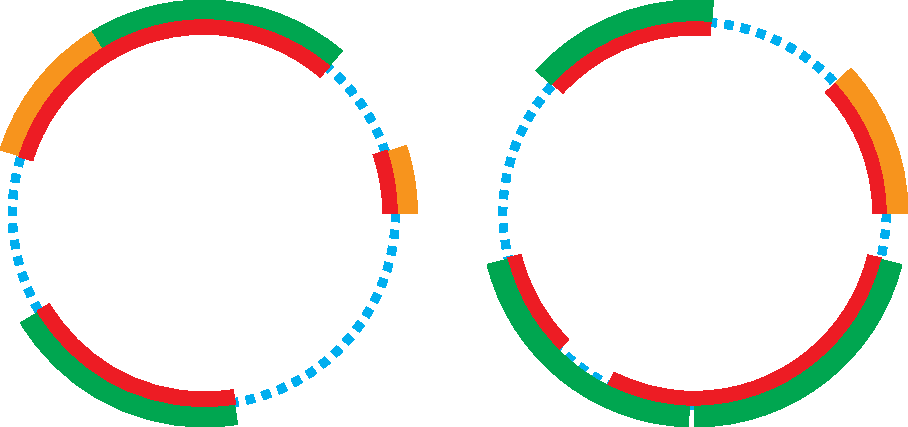
\includegraphics[scale = 0.6]{chapters/opg-ext/figures/mopglr_shrink-new-eps-converted-to.pdf}
    \caption{An \opglr problem and an associated optimal solution. The 
		problem has two perimeters and $t = 2$ with $n_1$=3, $n_2$=5, 
		$a_1$=5, $a_2$=8. The boundaries are shown as circles for ease of 
		illustration.
		%, which does not affect the computation or the solution.
		}
		\label{fig:opgext-opglrm}
\end{figure}

Shifting our attention to \opgmc, Fig.~\ref{fig:opgext-opgmc} illustrates the 
structure of an optimal solution to a problem with three types of robots 
with capacities and costs being $\ell_1=11, c_1=2$, $\ell_t=30, 
c_2=4$, and $\ell_3=55, c_3=7$, respectively. In this case, the majority 
of the deployed robots are of type $2$ with $\ell_2=30, c_2=4$. Only one 
type $1$ and one type $3$ robots are used. The four perimeter segments are 
covered by three robot groups. 
%
%To clearly illustrate the solution structure, the combined coverage of each 
%robot group runs beyond the counterclockwise direction of the corresponding 
%segments being covered (e.g., the counterclockwise end of the orange segment 
%is inside a gap). 
%
The only type $3$ robot guards (the purple segment) across two different 
perimeter segments. Coverage length adjustment is also performed to avoid 
the unnecessary coverage of some gaps. 

\begin{figure}[!ht]
    \centering
    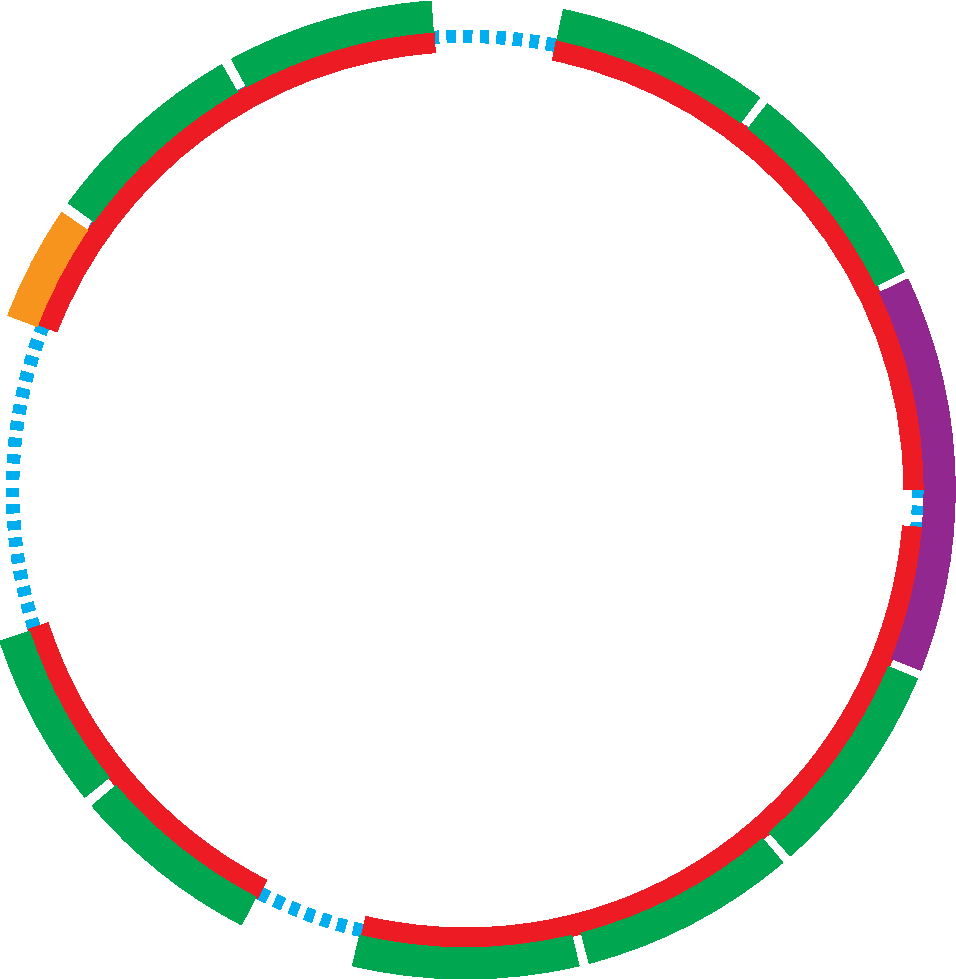
\includegraphics[scale = 0.4]{chapters/opg-ext/figures/opgmc-new-t-eps-converted-to.pdf}
    \caption{An \opgmc problem and an associated optimal solution. The 
		problem has four (red) perimeter segments and three types of robots
		with $\ell_1=11, c_1=2$ (orange), $\ell_t=30, c_2=4$ (green), 
		and $\ell_3=55, c_3=7$ (purple), respectively.}
		\label{fig:opgext-opgmc}
\end{figure}

\subsection{A Robotic Guarding and Patrolling Application}
In this subsection, as a potential application, the DP algorithms for 
\opglr and \opgmc are employed to solve the problem of securing the 
perimeter of the Edinburgh castle, an example used in 
\cite{FenHanGaoYu19RSS}. As shown in Fig.~\ref{fig:opgext-castle} (minus 
the orange and green segments showing the solutions), the central 
region of the Edinburgh castle has tall buildings on its boundary 
(the blocks in brick red); these parts of the boundary are the gaps 
that do not need guarding. In the figure, the top sub-figure shows 
the optimal solution for an \opglr instance and an \opgmc instance with 
a total of $11$ robots. The bottom sub-figure is a slightly updated 
\opgmc instance with slightly higher $c_2$. 
\begin{figure}[!ht]
    \centering
    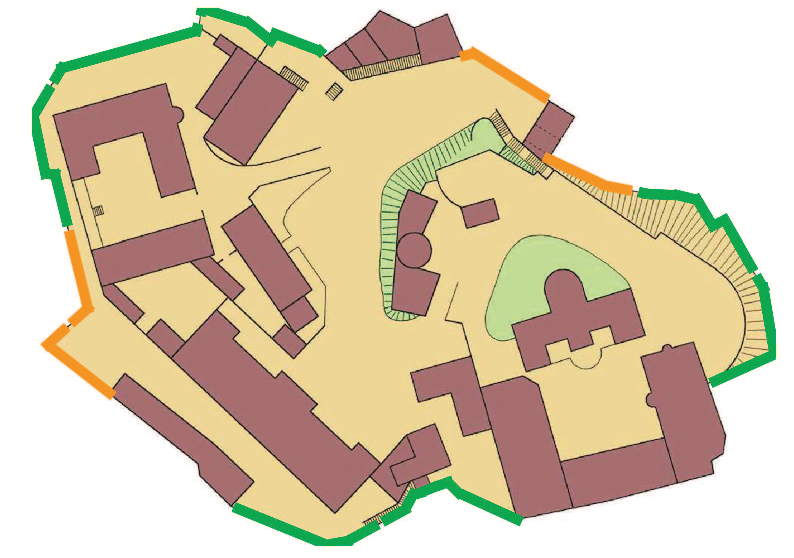
\includegraphics[scale = 0.5]{chapters/opg-ext/figures/opglr-castle-thin-eps-converted-to.pdf}
    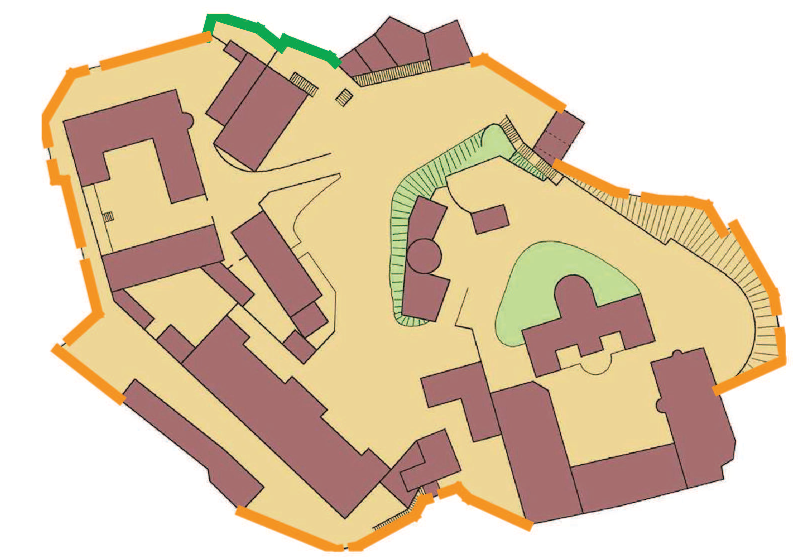
\includegraphics[scale = 0.5]{chapters/opg-ext/figures/opgmc-castle-thin-eps-converted-to.pdf}
    \caption{[left] \opglr solution with $n_1 = 4, n_2 = 7, 
		c_1:c_2 = 2:3$ and \opgmc solution with $\ell_1 = 150, 
		c_1 = 100, \ell_2 = 225, c_2 = 145$, and total boundary $3058$. Cost 
		of \opgmc solution is $1415$.
		[right] \opgmc solution with $\ell_1 = 150, c_1 = 100, \ell_2 = 
		225, c_2 = 155$. Cost of solution ($13$ type $1$, $1$ type $2$) is 
		$1455$.
		%
		In both solutions, covers by type $1$ (resp., 
		type $2$) robots are shown in orange (resp., green).
		%, which does not affect the computation or the solution.
		}
		\label{fig:opgext-castle}
\end{figure}

It can be observed that the results, while having non-trivial structures, 
make intuitive sense. For the top sub-figure, solutions to both \opglr 
and \opgmc (because robot with larger capacity is slightly lower in 
relative cost) use mainly higher capacity robots to cover longer perimeter 
segments and use the lower capacity robots mostly fillers. The solution 
covers a small gap at the bottom. For the bottom sub-figure, while only 
small changes are made to the cost, because the longer segment is more 
expensive to use now, the first type of robot is used mainly. 

\subsection{Computational Performance}
With Section~\ref{sec:opgext-algorithm} fully establishing the correctness and 
asymptotic complexity of the pseudo-polynomial time algorithms, here, the 
running time of these algorithms are experimentally evaluated. In doing 
so, the main goal is demonstrating that, despite the hardness of \opglr 
and \opgmc, the proposed algorithms could solve the target problems under 
reasonably broad settings in a scalable way. For results presented in 
this subsection, each data point is an average over 10 randomly generated 
instances. 

The first two numerical evaluations (Table~\ref{tab:opgext-opglr} and 
Table~\ref{tab:opgext-mopglr}) focus on the running times of the pseudo-polynomial 
time algorithms for \opglr over single and multiple perimeters, 
respectively. In these two tables, $t$ and $q$ are the number of types 
and the number of segments, respectively. For each type $\tau$, a 
capacity ($a_{\tau}$) is randomly sampled as an integer between $1$ and 
$100$, inclusive. The number of robots available for each type ($n_{\tau}$) 
is sampled uniformly between $5$ and $15$, inclusive. For the multiple 
perimeters case, the parameter $m$ represents the number of perimeters for 
a given instance.

For the single perimeter case (Table~\ref{tab:opgext-opglr}), the results show 
that the pseudo-polynomial time algorithm is effective for up to five 
types of robots, for dozens of robots. We expect a more efficient 
(e.g., C++ based) implementation should be able to effectively handle 
up to five types of robots with the total number of robots being around 
a hundred, on a typical PC. This is likely sufficient for many practical 
applications which have limited types and numbers of robots. Since the 
algorithm has exponential dependency on $t$, it becomes less efficient 
for larger $t$ as expected.  

\begin{table}[htbp]
	\centering
	\begin{tabularx}{\columnwidth}{|c|X|X|X|X|X|X|}
		\hline
%		\renewcommand{\arraystretch}{0.99}
		\diagbox{$t$}{$q$}&  \quad 5 &   \quad 10 &\quad 20& \quad 30 & \quad 40&\quad 50 \\
		\hline
		\renewcommand{\arraystretch}{1.05}
		2&0.022 &0.044 &0.131 &0.208 &0.326 &0.516 \\\hline
        3&0.281 &0.714 &1.670 &2.577 &4.107 &4.708 \\\hline
        4&5.504 &16.07 &41.68 &71.55 &109.9 &138.9 \\\hline
        5&29.53 &75.60 &243.6 &443.4 &528.0 &725.0 \\\hline
	\end{tabularx}
	\caption{Running time in seconds used by the DP algorithm for \opglr over 
	a single perimeter.
	}
	\label{tab:opglr}
\vspace*{-1mm}
\end{table}

Table~\ref{tab:opgext-mopglr} illustrates the running time of the DP algorithm for 
\opglr over multiple perimeters. As can be readily observed, the impact of 
the number of perimeters $m$ on the running time is relatively small; the 
number of robot types is still the determining factor for running time. In 
this case, our proposed solution is effective for $t$ up to $4$ and starts to 
slow down a robot types become larger than $4$. 
\begin{table}[htbp]
	\centering
	\renewcommand{\arraystretch}{1.05}
    \begin{tabularx}{\columnwidth}{|c|X|X|X|X|X|X|}
        \hline
        {\multirow{2}{*}{\diagbox{$m$}{$q$}} }&\multicolumn{2}{c|}{10}&\multicolumn{2}{c|}{20}&\multicolumn{2}{c|}{30} \\
        \cline{2-7}
         &\,\,\,$t$=3 & $\,\,\,t$=4& $\,\,\,t$=3 & $\,\,\,t$=4& \,\,\,$t$=3  & \,\,\,$t$=4\\
        \hline
        2&3.148 &133.2 &7.077 &198.4 &10.33 &260.0 \\\hline
        3&4.828 &194.1 &10.125 &290.6 &15.52 &376.7 \\\hline
        4&6.131 &256.8 &12.485 &381.3 &19.75 &514.3 \\\hline
        5&7.622 &321.7 &15.355 &476.2 &24.31 &605.8 \\\hline
    \end{tabularx}
    \caption{Running time in seconds used by the DP algorithm for \opglr over multiple perimeters.}
    \label{tab:mopglr}
\vspace*{-1mm}
\end{table}

Table~\ref{tab:opgext-opgmc} provides performance evaluation of \opgmcdp. Since 
there is no difference between single and multiple perimeters for \opgmc,
only problems with single perimeters are attempted. Here, for each robot 
type, the cost is an integer randomly sampled between $1$ and $20$, and 
the capacity is computed as five times the cost plus a random integer 
between $1$ and $20$. In the table, $L = \partial R$, the total length 
of the entire boundary. 
%
Given \opgmc's lower computational complexity, the DP algorithm, 
\opgmcdp, can effectively deal with over a few hundred types of robots 
with ease. 
\begin{table}[!ht]
	\centering
	\renewcommand{\arraystretch}{1.04}
    \begin{tabularx}{\columnwidth}{|c|X|X|X|X|X|X|}
        \hline
        \multirow{2}{*}{\diagbox{$t$}{$L$}} & 
        \multicolumn{2}{c|}{$10^2$}&\multicolumn{2}{c|}{$10^4$} &\multicolumn{2}{c|}{$10^6$} \\
        \cline{2-7}
        &$q$=20&$q$=50&$q$=20&$q$=50&$q$=20&$q$=50\\
        \hline
        3&0.006 &0.064 &0.041 &0.098 &3.040 &3.144 \\\hline
        10&0.005 &0.066 &0.094 &0.155 &9.423 &9.409 \\\hline
        30&0.009 &0.070 &0.261 &0.320 &26.10 &28.59 \\\hline
        100&0.014 &0.077 &0.910 &0.969 &91.28 &93.20 \\\hline
        300&0.030 &0.091 &2.652 &2.938 &275.6 &270.7 \\\hline
    \end{tabularx}
    \caption{Running time in seconds used by \opgmcdp algorithm.}
    \label{tab:opgext-opgmc}
\end{table}
\vspace*{-1mm}
\begin{comment}
    Application 1: for a single large region with a perimeter that may be viewed as straight line segments locally, we want to deploy multiple types of robots with different sensing radius. The goal is to ensure full coverage of the perimeter. Both problems formulations can be used. 

This also raises a related problem: what if we want to use discs to cover perimeter when a segment cannot be treated as straight lines? Can we also do tiling somehow? 

Another question: if we just use the same number of robots as used in an optimal cover to do a random feasible tiling, what would be the worst sub-optimality ratio? 

Application 2:  a multi-region application?
\end{comment}

\subsection{Conclusion and Discussions}\label{sec:opgext-conclusion}
In this section, we investigate two natural models of optimal perimeter 
guarding using heterogeneous robots, where one model (\opglr) limits 
the number of available robots and the second (\opgmc) seeks to 
optimize the total cost of coverage. 

These formulations have many potential applications. One application 
scenario we envision is the deployment of multiple agents or robots 
as ``emergency responders'' that are constrained to travel on the 
boundary. An optimal coverage solution will then translate to minimizing 
the maximum response time anywhere on the perimeter (the part that 
needs guarding). The scenario applies to \opg, \opglr, and \opgmc. 

Another application scenario is the monitoring of the perimeter 
using robots with different sensing capabilities. A simple heterogeneous 
sensing model here would be robots equipped with cameras with different 
resolutions, which may also be approximated as discs of different radii. 
The model makes sense provided that the region to be covered is much 
larger than the sensing range of individual robots and assuming that the 
boundary has relatively small curvature as compared to the inverse of the 
radius of the smallest sensing disc of the robots. For boundary with 
relatively small curvature, our solutions would apply well to the sensing 
model by using the diameter of the sensing disc as the 1D sensing range. 
As the region to be covered is large, covering the boundary will require
much fewer sensors than covering the interior. 


On the computational complexity 
side, we prove that both \opglr and \opgmc are NP-hard, with \opglr 
directly shown to be strongly NP-hard. This is in stark contrast to 
the homogeneous case, which admits highly efficient low polynomial 
time solutions \cite{fenghangaoyu2019efficient}. The complexity study also 
establishes structural similarities between these problems and 
classical NP-hard problems including \tpart, \ttkp, and \subsetsum.

On the algorithmic side, we provide methods for solving both \opglr 
and \opgmc exactly. For \opglr, the algorithm runs in pseudo-polynomial 
time in practical settings with limited types of robots. In 
this case, the approach is shown to be computationally effective. 
For \opgmc, a pseudo-polynomial time algorithm is derived for the 
general problem, which implies that \opgmc is weakly NP-hard. In 
practice, this allows us to solve large instances of \opgmc. We 
further show that a polynomial time algorithm is possible for 
\opgmc when the types of robots are fixed. 

With the study of \opg \cite{fenghangaoyu2019efficient} for homogeneous and 
heterogeneous cases, some preliminary understanding has been 
obtained on how to approach complex 1D guarding problems. 
Nevertheless, the study so far is limited to {\em one-shot} settings
where the perimeters do not change. In future research, we would like 
to explore the more challenging case where the perimeters evolve 
over time, which requires the solution to be dynamic as well. Given 
the results on the one-shot settings, we expect the dynamic setting
to be generally intractable if global optimal solutions are desired, 
potentially calling for iterative and/or approximate solutions. 

We recognize that our work 
does not readily apply to a visibility-based sensing model, which is also 
of interest. Currently, we are also exploring covering of the interior
using range-based sensing. As with the OPG work, we want to push for 
optimal or near-optimal solutions when possible.
\vspace*{-1mm}

